This chapter will present the results of calculations using each of the decusping methods described in the previous chapter.  First, results for the polynomial and subplane collision probabilities methods will be presented.  The subplane collision probabilities results are presented as two sets of data: one with just subplane (axial correction only) and one with both subplane and CP (axial and radial), allowing the difference in magnitude between the axial and radial effects of the rod to be determined.  These methods were tested using the VERA Progression Problems \cite{VERAProgressionProblems}, a series of benchmark problems based on the Watts Bar Unit 1 pressurized water reactor (PWR) that provide realistic test cases for the 2D/1D methods.  The control rods in these models were moved to various locations that stress the mesh typically used by MPACT to solve these problems, allowing the benefit of the decusping techniques to be clearly seen.  For some of these problems, detailed 3D power distributions were generated using the Monte Carlo code KENO-VI \cite{SCALE6.2}, allowing for comparisons of the decusping methods with both refined MPACT meshes and Monte Carlo reference solutions.

In the second half of the chapter, results for the subray method of characteristics will be presented.  The first set of results come from the 1D prototype code discussed in Section \ref{ss:1dcode}.  This code provided a quick implementation to show that it was worth pursuing the method in a full-scale transport code.  After this, results from MPACT's implementation of subray MOC will be presented for both 2D and 3D problems.  These results will be compared to refined mesh solutions in MPACT as well as the polynomial and subplane collision probabilities solutions to determine the relative accuracy of each of these methods.  All subray MOC results will use the C5G7 benchmark problems \cite{EELewisC5G72003,EELewisC5G7extended2005}.  Because these problems have specified macroscopic cross sections, some of the complexities of cross section processing and shielding calculations for subray MOC can be deferred to later research while still examining the accuracy and performance of subray MOC compared with other solutions to the rod cusping problem.

\section{VERA Problem 4}\label{s:vera4}

\begin{figure}[h]\label{f:p4layout}
    \centering
    \subfigure{\label{f:p4radial}
        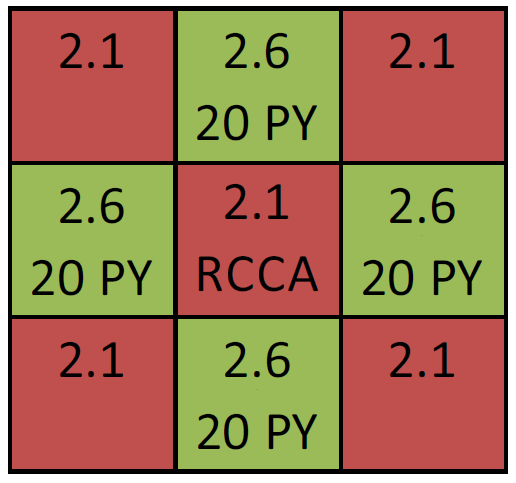
\includegraphics[width=0.4\textwidth]{p4a_layout.png}
    }
    ~
    \subfigure{\label{f:p4axial}
        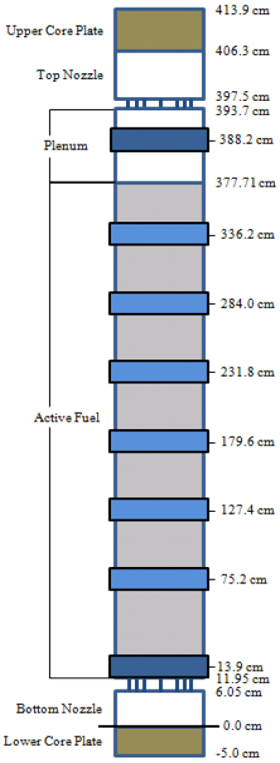
\includegraphics[width=0.3\textwidth]{wb_3d_assembly.png}
    }
    \caption{VERA Problem 4 radial (left) and axial (right) layouts}\label{f:p4}
\end{figure}

VERA Progression Problem 4 is composed of a 3x3 set of Westinghouse 17$\times$17 fuel assemblies with an active fuel height of 365.76 cm and a control bank in the center assembly.  The radial layout of the problem is shown in Figure \ref{f:p4radial}, and the axial layout of each assembly is shown in Figure \ref{f:p4axial}.  The control rods were placed at an axial elevation of 257.9 cm above the core plate, about one third inserted into the core.  The rod in the original problem specification is made of AIC with a \bfc{} follower and a stainless steel tip.  First, results will be presented which use several difference uniform rods to simplify the analysis, then results will be presented with the heterogeneous rod.  Lastly, a differential rod worth developed with the heterogeneous rod is shown with comparisons to KENO-VI reference solutions at regular intervals along the curve.

\subsection{Homogeneous Control Rods}

For the reference solution, 58 MOC planes were used with 49 of them in the active fuel region.  It was also ensured that the end of the control rods were exactly aligned with one of the MOC plane boundaries.  The cases with decusping methods used the same mesh, but with the 2 MOC planes around the tip of the control rod merged into a single plane to introduce cusping effects.  The accuracy and convergence data for these cases are shown in Table \ref{t:homoDecusp}.

\begin{table}[ht]
    \centering
    \caption[VERA Problem 4 Homogeneous Rod Results]{Comparison of Rod Decusping Methods in MPACT for VERA Progression 
        Problem 4 for Homogeneous Control Rods}
    \resizebox{\textwidth}{!}{\begin{tabular}{l l S[table-format=3.1,table-number-alignment=left] 
            S[table-format=1.2,table-number-alignment=left] 
            S[table-format=2.2,table-number-alignment=left] 
            S[table-format=2.1,table-number-alignment=left] l}\toprule
        Rod & \multirow{2}{*}{{Case}} & {\keff{}} & 
        \multicolumn{2}{l}{{Pin Power 
                Differences}} & \multirow{2}{*}{{2D/1D Iterations}} & {Runtime}\\
        Material & & {Difference (pcm)} & {RMS} & {Max} &  & {(Core-Hours)} \\\midrule
        \multirow{5}{*}{AIC}      & Reference        & {--}  &    {--} &     {--} & 15 & 19.6 \\
                                  & No treatment     & -29.5 & 1.53\% & 11.84\% & 12 & 14.7 \\
                                  & Polynomial       &  -0.3 & 0.44\% &  4.08\% & 12 & 14.3 \\
                                  & Subplane         & -11.5 & 0.73\% &  8.21\% & 12 & 14.2 \\
                                  & Subplane + CP    &  -5.6 & 0.37\% &  4.25\% & 12 & 15.3\\\midrule
        \multirow{5}{*}{\bfc{}}   & Reference        & {--}  &    {--} &     {--} & 15 & 16.9 \\
                                  & No treatment     & 112.0 & 6.98\% & 69.37\% & 12 & 12.7 \\
                                  & Polynomial       & 112.6 & 6.89\% & 66.73\% & 12 & 12.1 \\
                                  & Subplane         & -17.9 & 1.14\% & 11.36\% & 13 & 15.2 \\
                                  & Subplane + CP & -11.0 & 0.69\% &  6.37\% & 12 & 13.4 \\\midrule
        \multirow{5}{*}{Tungsten} & Reference        & {--}  & {--}   &      {--} & 15 & 23.5 \\
                                  & No treatment     &  -8.4 & 0.37\% &  3.37\% & 12 & 15.5 \\
                                  & Polynomial       &  -4.4 & 0.24\% &  2.72\% & 12 & 14.5 \\
                                  & Subplane         &   1.6 & 0.07\% &  0.60\% & 12 & 13.9 \\
                                  & Subplane + CP    &  -0.9 & 0.06\% &  0.94\% & 12 & 15.6 \\\bottomrule
    \end{tabular}}
    \label{t:homoDecusp}
\end{table}

The ``No Treatment'' cases show the magnitude of the cusping effects for each of the rod types.  The largest cusping errors occur for the \bfc{} rod, which is a strong thermal absorber.  For this rod, the polynomial treatment has very little effect, leaving large errors in the solution.  The subplane method reduces the error in \keff{} to an almost negligible -18 pcm, but still leaves significant power distribution errors of 1.14\% RMS and 11.36\% Max.  Introduing the 1D CP calculations brings the maximum error below 7\%.  These results indicate that the polynomial method is not capable of accurately resolving the \bfc{} rod.  Because it is a strong thermal absorber, smearing the rod material throughout the plane at all introduces large errors that cannot be correct just by reducing the volume fraction.  The subplane-based methods are both able to resolve the rod more accurately since they actually modify the cross sections used in the CMFD and P$_3$ calculations.

For the AIC rod, the polynomial correction performs much better than for the \bfc{} rod, reducing the maximum error from 12\% to 4\%.  The subplane treatment only reduces the error to 8.21\%, while adding the CP calculations reduces the errors to about the same point as the polynomial treatment.  The AIC rod has resonance absorption and is not as strongly absorbing in the thermal energy ranges as the \bfc{} rod, causing some differences in behavior of these methods.  The polynomial method does a better job with the AIC rod since the complex effects are accounted for in the polynomial generation.  However, the subplane treatment does not perform well since it does nothing to account for the radial effects of the AIC rod.  For both rod types, the subplane treatment with radial CP calculations performs well since it is able to capture both radial and axial effects of the rod.

For the tungsten rod, the errors are not nearly as high as for the AIC or \bfc{} rods.  However, the subplane-based treatments still perform significantly better than the polynomial treatment, bringing the \keff{} error to negligible levels and reducing the maximum power errors under 1\%.

For all 3 rod types, Table \ref{t:homoDecusp} also shows the convergence and runtime data for each calculation.  The decusping treatments consistently converge in fewer iterations than the reference.  This is due to the fact that the reference has an additional thin MOC plane that the other cases do not have.  This thin plane requires underrelaxation for 2D/1D to converge, causing a small increase in the number of 2D/1D iterations required.  Because of the difference in iterations, all decusping methods also require less runtime by about 25\% on average.  The subplane-based methods are generally a bit slower than the polynomial method, despite requiring the same number of 2D/1D iterations.  The reason for this is that the subplane-based methods modify the CMFD system, which results in more CMFD inner iterations to converge during each outer 2D/1D iteration.  This increases the total runtime of the problem even though 2D/1D itself converges the same.  However, in most cases the trade-off between runtime and accuracy would favor the use of the subplane-based 

\subsection{Heterogeneous Control Rod}

Next, the same set of results can be shown again, but with the heterogeneous rod.  The same 58-plane reference mesh was used for these results.  However, the decusping cases have only 55 planes instead of 57.  Three additional planes are eneded in the reference case to account for all three material interfaces in the heterogeneous rod: \bfc{}/AIC, AIC/SS, and SS/moderator.  The decusping methods are applied at all three of these locations simultaneously, with the exception of the SS/moderator interface for the polynomial decusping since there is no SS polynomial data.  The results are shown in Table \ref{t:hetDecusp}.

\begin{table}[ht]
    \centering
    \caption[VERA Problem 4 Heterogeneous Rod Results]{Comparison of Rod Decusping Methods in MPACT for VERA Progression 
        Problem 4 for Heterogeneous Control Rod}
    \begin{tabular}{l S[table-format=2.1,table-number-alignment=left] l 
            S[table-format=2.3,table-number-alignment=left] l l}\toprule
        \multirow{2}{*}{Case} & {\keff{}} & \multicolumn{2}{l}{{Pin Power 
                Differences}} & \multirow{2}{*}{{2D/1D Iterations}} & {Runtime}\\
        & {Difference (pcm)} & {RMS} & {Max} &  & {(Core-Hours)} \\\midrule
        Reference        &  {--} &    {--} &     {--} & 15 & 16.6 \\
        No treatment     & -45.9 & 2.43\% & 20.45\% & 12 & 13.8 \\
        Polynomial       &  -2.5 & 0.46\% &  5.07\% & 12 & 13.0 \\
        Subplane         & -17.3 & 1.10\% & 11.77\% & 13 & 14.9 \\
        Subplane + CP    &  -5.5 & 0.42\% &  3.87\% & 12 & 14.7 \\\bottomrule
    \end{tabular}
    \label{t:hetDecusp}
\end{table}

With no treatment, the maximum error is over 20\%.  The polynomial method performs wells, reducing the error to about 5\%, with an RMS power error under 0.5\% and \keff{} error of -2.5 pcm.  This behavior is consistent with what is expected based on the homogeneous results.  The primary location of rod cusping effects is at the AIC/SS interface, and the errors obtained from the polynomial decusping method are comparable to those observed in the homogeneous AIC rod calculations.  Following this trend, the subplane treatment without radial CP does not perform as well as the polynomial treatment, reducing the maximum error to just under 12\%.  Finally, the subplane treatment with radial CP generates the most accurate results, with a maximum power error under 4\%.  This method makes no assumptions about which materials are next to each other, can handle all three control rod materials, and accounts for both radial and axial effects of the rod, making it the most consistent and accurate of the methods across a variety of cases.

The trends in the convergence and runtime data are similar to those observed with the homogeneous rods.  The decusping treatment calculations take fewer 2D/1D iterations because fewer thin planes are used in the model, requiring less underrelaxation than the reference case.  Furthermore, some increase in runtime is seen in the subplane-based methods over the polynomial method due to changes in the convergence of the CMFD system during each 2D/1D iteration.  The CP calculations themselves are negligible since they consist only of inverting an 8$\times$8 matrix for each energy group, which can be done very quickly.  Again, the trade-off between runtime and accuracy for this problem favors using the subplane treatment with radial CP if the fine mesh solution's accuracy is not required.

\subsection{Differential Rod Worth Curve}

\begin{figure}[h]
    \centering
    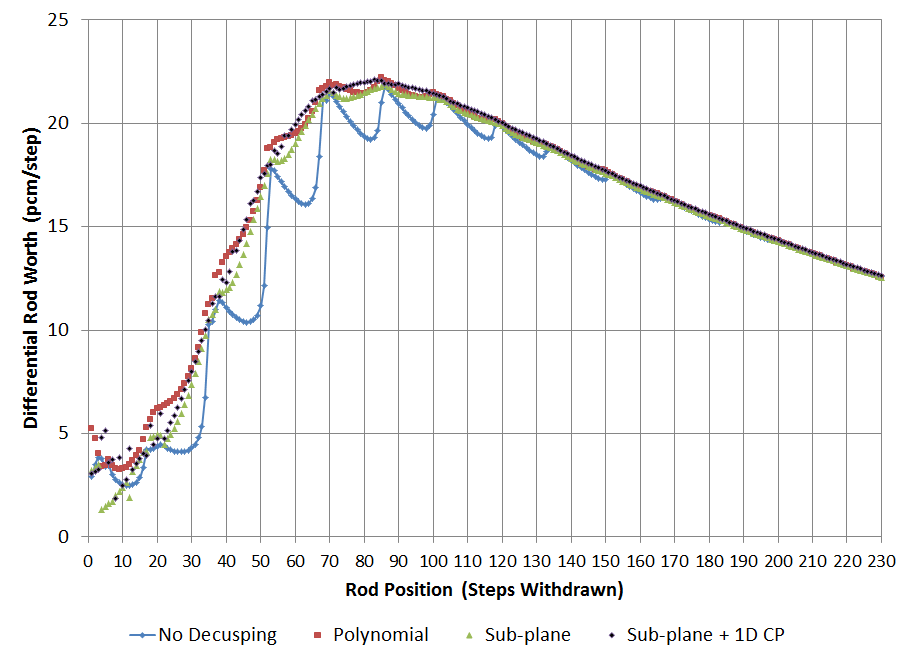
\includegraphics[width=\textwidth]{../../figs/differentialRodworth.png}
    \caption{Differential rod worth curves for MPACT decusping 
        techniques.}\label{f:rodworth}
\end{figure}

To show the effectiveness of each decusping technique as the rod moves upward through the reactor, a differential rod worth curve was developed for each method.  This curve is shown in Figure \ref{f:rodworth}.  With no decusping method, the errors in the rodworth approach 50\% at some positions.  The polynomial treatment greatly reduces these errors, but does not fully smooth the curve.  Especially near the peak of the curve, some oscillation about the true solution can be seen when using the polynomial treatment.  The subplane treatment behaves similarly to the polynomial treatment, but with slightly larger errors in most places.  Finally, adding the radial CP calculations generates a smooth curve at almost every rod position.

The exception to the good behavior of the subplane + CP method occurs when the rod is almost fully inserted.  At such positions, all methods fail to produce a smooth rod worth curve due to the severe power shape.  The polynomial method is always limited in its ability to resolve the partially inserted rod if the local power shape differs significantly from the one with which the polynomial data was generated.  The subplane-based treatments struggle with the fully inserted rod because each subplane in an MOC plane uses the same MOC solution data for the CMFD and P$_3$ solutions.  In the cases where MOC planes are near both the control rod tip and the boundary of the problem, the radial solution is changing more quickly than normal and cannot be resolved as well by the subplane scheme.

\subsection{KENO-VI Comparisons}

\begin{table}[h]
    \centering
    \caption{Average Differences between MPACT and KENO-VI for VERA Problem 
        4}\label{t:keno}
    \sisetup{separate-uncertainty=true,table-text-alignment=left,table-number-alignment=left}
    \begin{tabular}{l l 
            S[table-format=3.1,table-number-alignment=left] 
            S[table-format=1.3,table-number-alignment=left] 
            S[table-format=2.3,table-number-alignment=left]}\toprule
        \multirow{2}{*}{Cases} & \multirow{2}{*}{{Decusping Method}} & \multirow{2}{*}{{\keff{} 
                Difference}} & 
        \multicolumn{2}{l}{{Pin Power Difference}} \\
        &  &  & {RMS} & {Max} \\\midrule
        \multirow{4}{*}{Average}       & None              &   -24.9 &  5.380\% & 25.902\% \\
                                       & Polynomial        &    34.8 &  1.502\% &  8.957\% \\
                                       & Subplane          &    34.6 &  0.984\% &  4.597\% \\
                                       & Subplane + CP     &    41.4 &  0.763\% &  3.386\% 
        \\\midrule
        \multirow{2}{*}{Worst -- 20\%} & None              & -176.0 & 14.709\% & 63.929\% \\
                                       & Polynomial        & 13.9   &  3.344\% & 25.373\% \\
                                       & Subplane          & 9.6    &  1.921\% &  9.900\% \\
                                       & Subplane + CP     & 45.9   &  1.324\% &  4.921\% \\
        \midrule
        Fully Withdrawn                & --                & 40.5   & 0.34\%   & 1.493\% \\
        \bottomrule
    \end{tabular}
\end{table}

For the rod worth curves in the previous section, KENO-VI calculations were done in 10\% intervals along the curve, giving a total of 11 KENO-VI data sets that can be used as a reference for MPACT.  Each KENO-VI calculation was run for 500 inactive generations and 1000 active generations, with $5\times 10^6$ particles per generation, for a total of $5\times 10^9$ particles contributing to the final solution and statistics.  The uncertainty in the KENO-VI results was about 1 pcm for the eigenvalue and less than 0.3\% for the power distribution.  While the uncertainty in the power distribution is a bit higher than would normally be used, it is more than sufficiently converged to discuss the relative accuracy of rod cusping treatments.  For the first ten sets of KENO-VI data along the curve, each decusping method was compared.  Table \ref{t:keno} shows the average results for all 10 of these points, along with results for the worst of the 10, which occurs at 20\% (46 steps withdrawn) where the differential rod worth curve is steepest.  The table also shows a comparison for the 100\% withdrawn data set.  This final data set occurs for the tip of the control rod above the top of the active fuel, so there are no cusping effects.  This serves to give an idea of how accurate MPACT is compared to Monte Carlo when there are no control rod cusping effects.

The fully withdrawn case shows that when no cusping effects are present, MPACT can be expected to have less than 0.5\% RMS power difference and approximately 1.5\% maximum power difference compared with a Monte Carlo solution.  When cusping is introduced, these errors jump to around 25\% on average, with a maximum error over 60\%.  For both the average and maximum cases, the polynomial treatment compares worst with KENO-VI and the subplane treatment with 1D CP performs best, reducing the maximum power errors to about 5\% in the worst case scenario.  While these errors are still larger than desired for 2D/1D, they are much closer to acceptable levels than some of the 20-30\% errors observed in many calculations.  However, these KENO-VI comparisons do indicate that use of the polynomial decusping treatment should be restricted to specific cases in which it is known to perform well.  Using it for everything could easily and unknowingly result in unacceptably large errors in the 2D/1D solution.

\section{VERA Problem 5}

To demonstrate the behavior of the decusping methods on a full core problem, VERA Problem 5 was also run.  Problem 5 is the a beginning-of-cycle simulation of the Watts Bar Unit 1 PWR.  The model of this reactor uses the same axial layout shown in Figure \ref{f:p4axial} with the radial layout shown in Figure \ref{f:p5radial}.  For these calculations, Bank D was set to a position of 257.9 cm above the core plate while all other banks were fully withdrawn to 383.3125 cm, about 6 cm above the top of the active fuel.

Like Problem 4, the reference case was run with 58 planes while the decusping cases were run with 57 planes.  Radial decomposition was used with 16 cores per MOC plane.  This resulted in a slightly different number of cores for the reference case compared with the others, as seen in the Problem 4 calculations.  The accuracy and convergence results for the partially rodded plane are shown in Table \ref{t:p5decusp}.

\begin{figure}[h]
\centering
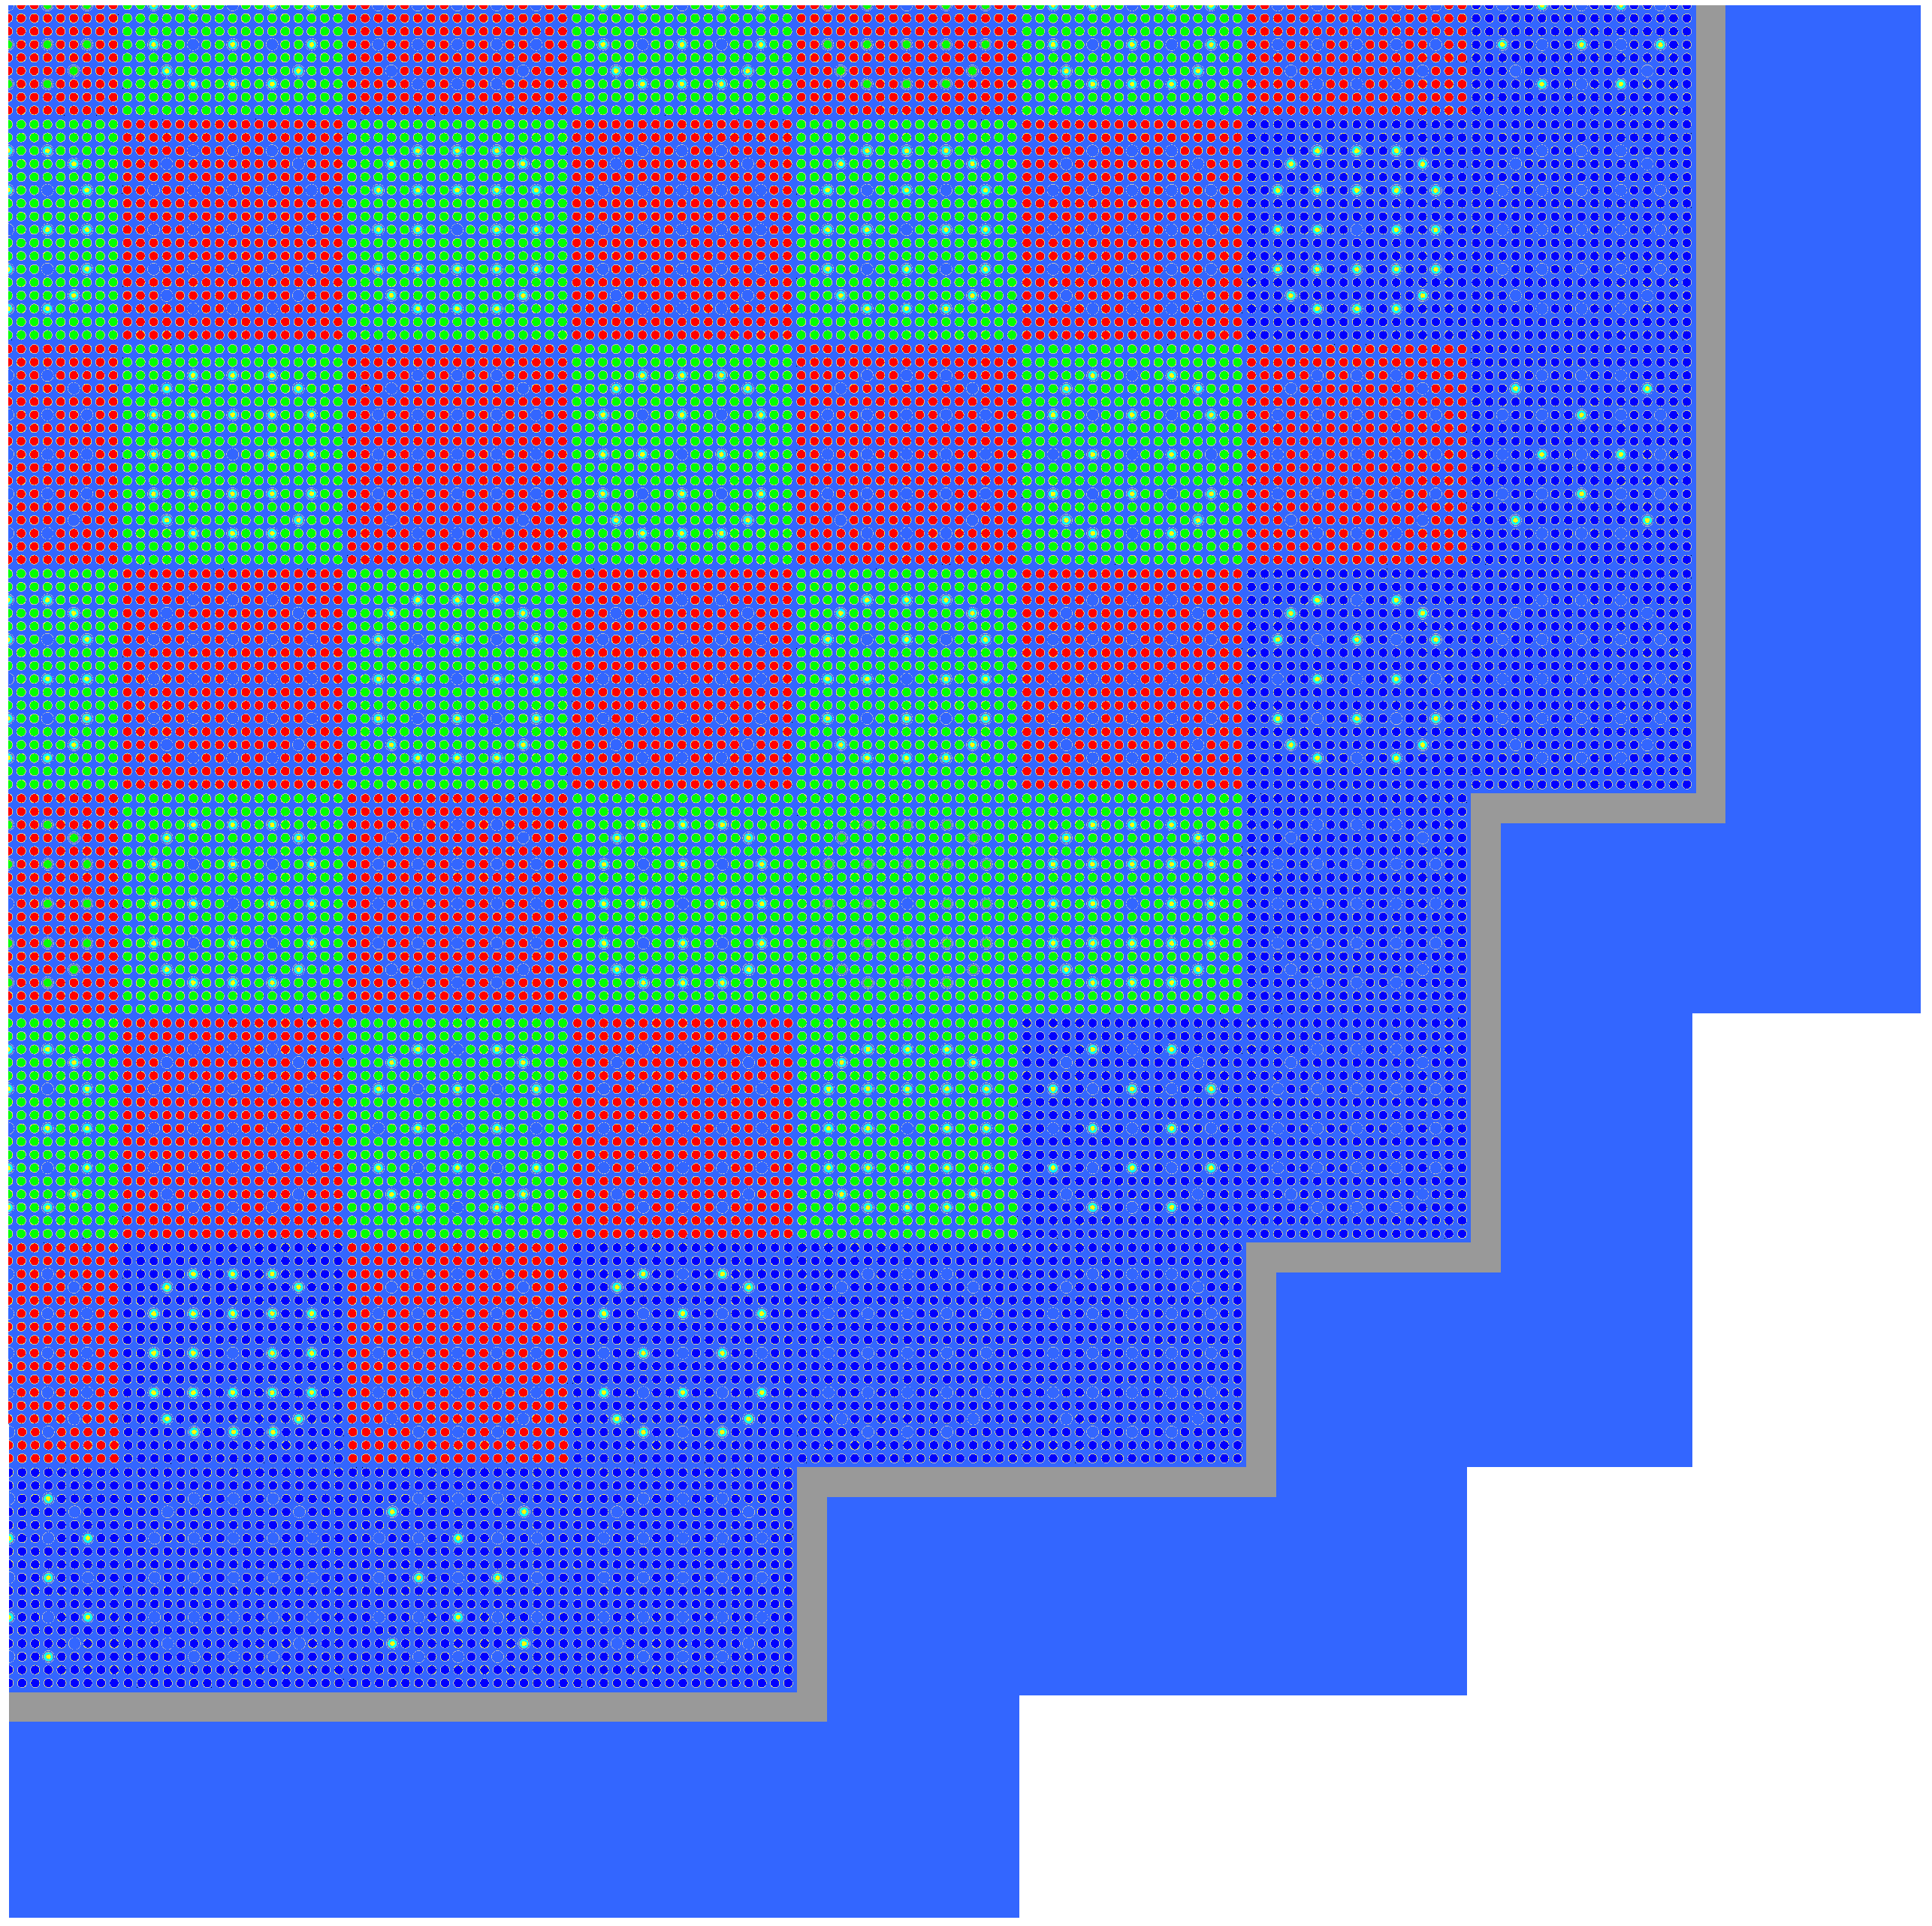
\includegraphics[width=0.48\textwidth]{p5_2D_baffle.png}
\hfill
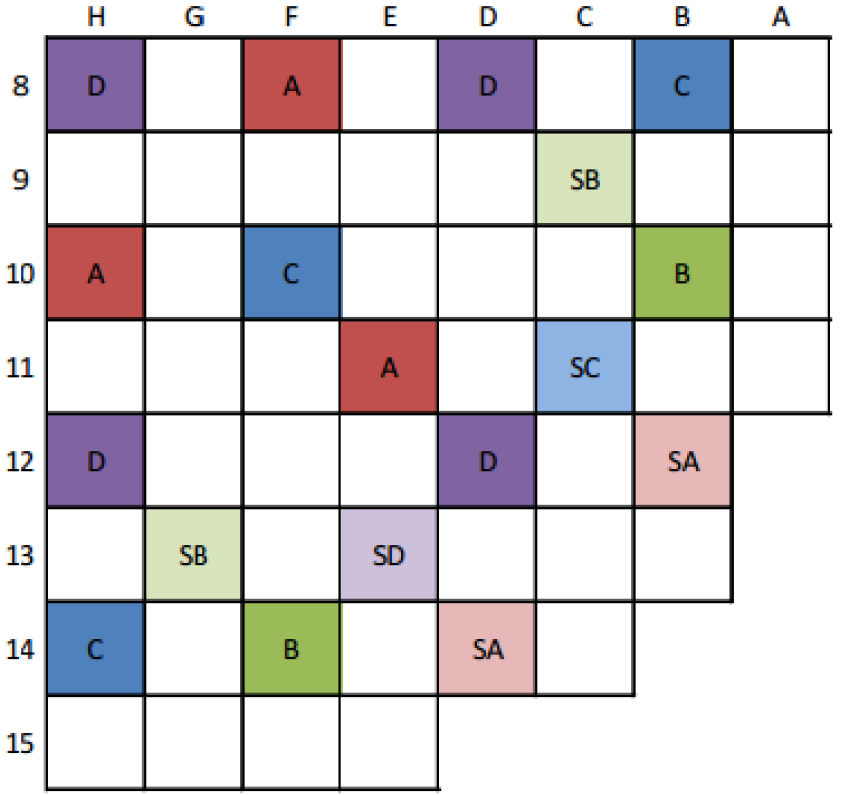
\includegraphics[width=0.48\textwidth]{WB1-cycle1-rodbank-layout.png}
\caption{VERA Problem 5 radial geometry (left) and rod bank positions (right)}\label{f:p5radial}
\end{figure}

\begin{table}[h]
\centering
\caption[VERA Problem 5 Decusping Results]{VERA Problem 5 decusping results for the partially rodded plane}\label{t:p5decusp}
\resizebox{\textwidth}{!}{
  \begin{tabular}{c c c c c c c}\toprule
    \multirow{2}{*}{Case} & \keff{} & \multicolumn{2}{c}{Pin Power Differences} & \multicolumn{2}{c}{Iterations} & Runtime\\
    & Difference (pcm) & RMS & Max & 2D/1D & CMFD & (Core-Hours) \\\midrule
    Reference        &  -- & --     & --      & 13 & 481 & 361.7 \\
    No Treatment     & -22 & 6.90\% & 30.55\% & 13 & 523 & 410.7 \\
    Polynomial       &  -5 & 1.15\% &  4.85\% & 13 & 463 & 373.7 \\
    Subplane         &  -5 & 2.09\% & 10.20\% & 13 & 499 & 399.0 \\
    Subplane + CP    &  -1 & 0.50\% &  2.74\% & 13 & 529 & 425.6 \\
    \bottomrule
  \end{tabular}
}
\end{table}

As seen in most variations of Problem 4, we see that the CP results are the best, with less than 3\% maximum error in the roded plane.  The maximum errors occur in the partially rodded assembly, as expected.  The sublpane decusping without the CP treatment is worse than in Problem 4, showing the importance of correctly treating the radial effects.  The runtime increase is also between 15\% and 20\% for the sublpane and CP decusping methods.  This is due primarily to two effects.  The first is that the convergence of the CMFD system can require more iterations using the subplane-based treatments, as discussed in the Problem 4 results.  The second effect is that there is an imbalance in the parallel partitioning of the CMFD system.  The parallel partitioning in MPACT is tied to MOC planes, so MOC planes with a larger number of subplanes will take longer to be solved than others, leaving some compute cores waiting on others to finish their calculations.  This effect would have also occurred some Problem 4, but is more significant in Problem 5 due to its larger size.  A more clever strategy for parallel decomposition would help to alleviate this imbalance and reduce the runtime of the subplane-based methods without any impact on their accuracy.

\section{C5G7 Results}

This section will focus on the results for the C5G7 benchmark problems for the subray method of characteristics.  First, 1D results generated by a simple prototype code will be presented, followed by 2D and 3D results from the 2D/1D code MPACT.  While the focus of this section is on subray MOC, the 2D and 3D results will also include the polynomial and subplane collision probabilities decusping techniques to show the accuracy of subray MOC compared with the other methods discussed already.

\subsection{1D Subray}

\begin{figure}[h]
    \centering
    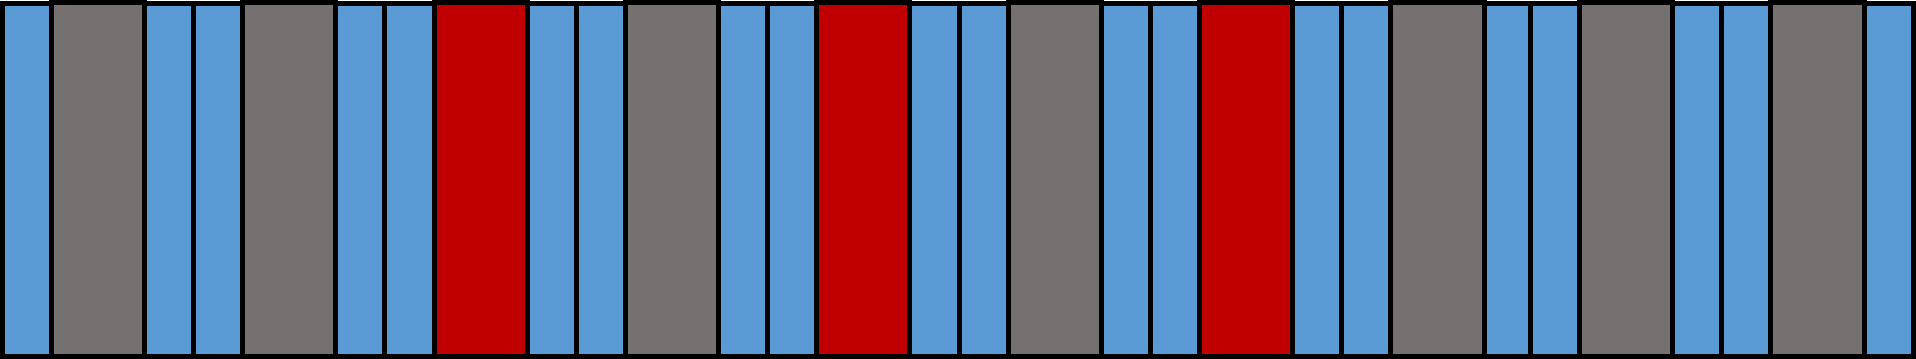
\includegraphics[width=\textwidth]{10pin-slab-geometry.png}
    \caption[Illustration of 1D MOC 10 Pin Geometry]{Illustration of 1D MOC 10 pin test geometry with materials fuel (grey), control rod/moderator mixture (red), and moderator (blue).}\label{f:10pin-geom}
\end{figure}

The 1D subray MOC results were generated using the code described in Section \ref{ss:1dcode}.  To show the effectiveness of subray MOC a small 10 pin problem, illustrated in Figure \ref{f:10pin-geom}, was used.  This smaller problem was used because the rods are closer together, making it more difficult to accurately resolve the rods, and to minimize runtime.  To show the effectiveness of the subray method, a series of eigenvalue calculates was performed with the control rod volume fraction varying from 100\% to 0\% to simulate a rod withdrawal.  This was done using traditional MOC and subray MOC to show the correction achieved by using subray MOC.  The reference solution for these calculations is generated by using the volume fractions to mix the fully rodded and unrodded solutions at each iteration and calculating the updated eigenvalue.  The results of these calculations are shown in Figure \ref{f:1d-subray-keff}.

\begin{figure}[h]
    \centering
    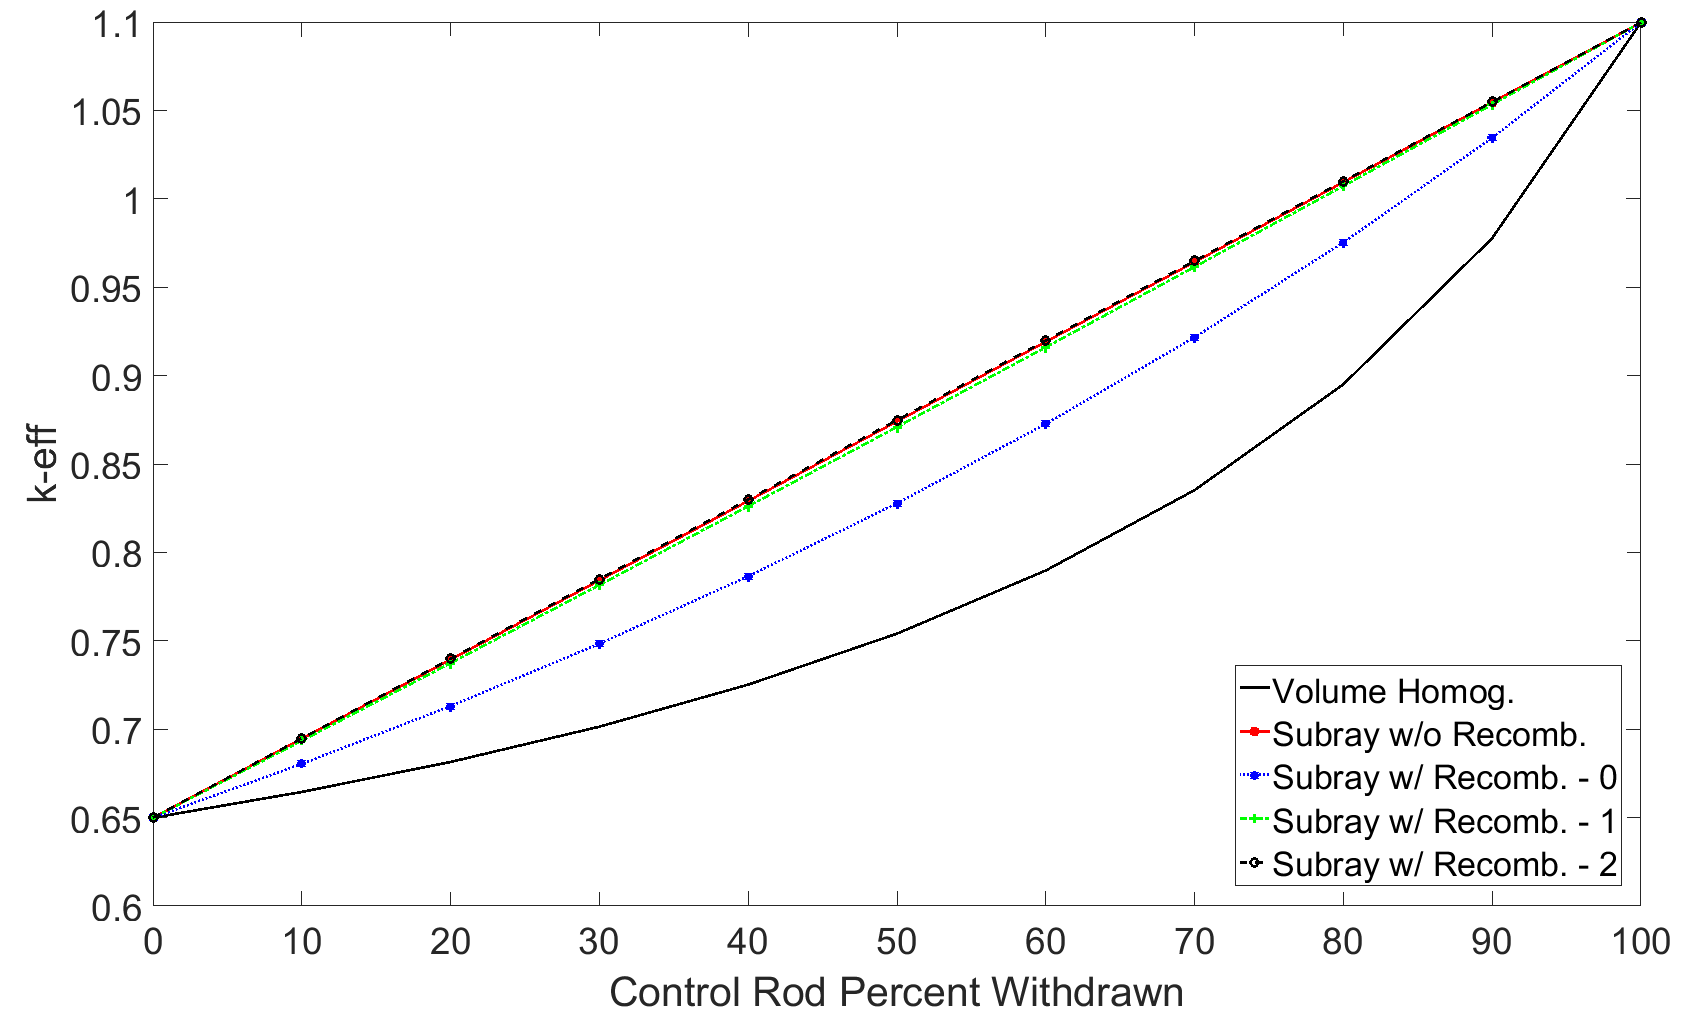
\includegraphics[width=0.8\textwidth]{keff_subray.png}
    \caption{Eigenvalue comparisons for 1D rod withdrawal}\label{f:1d-subray-keff}
\end{figure}

\begin{figure}[!htb]
    \centering
    \subfigure[Group 1]{
        \centering
        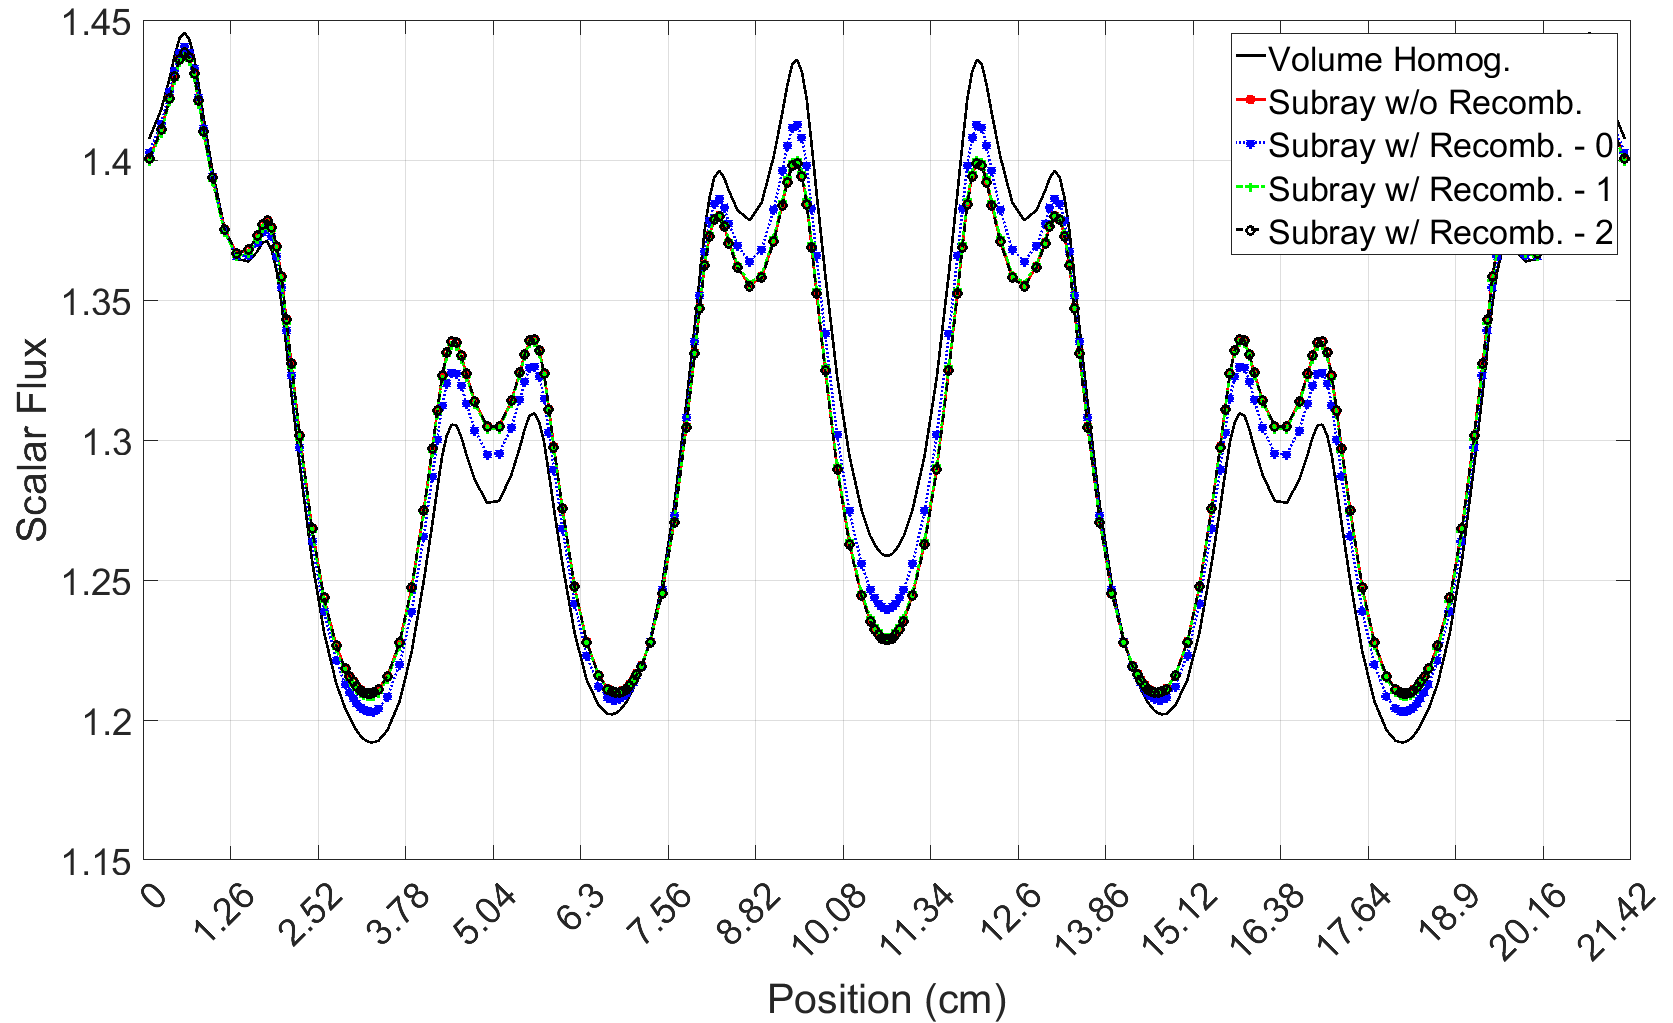
\includegraphics[width=\textwidth]{scalflux1.png}
    }
    ~
    \subfigure[Group 7]{
        \centering
        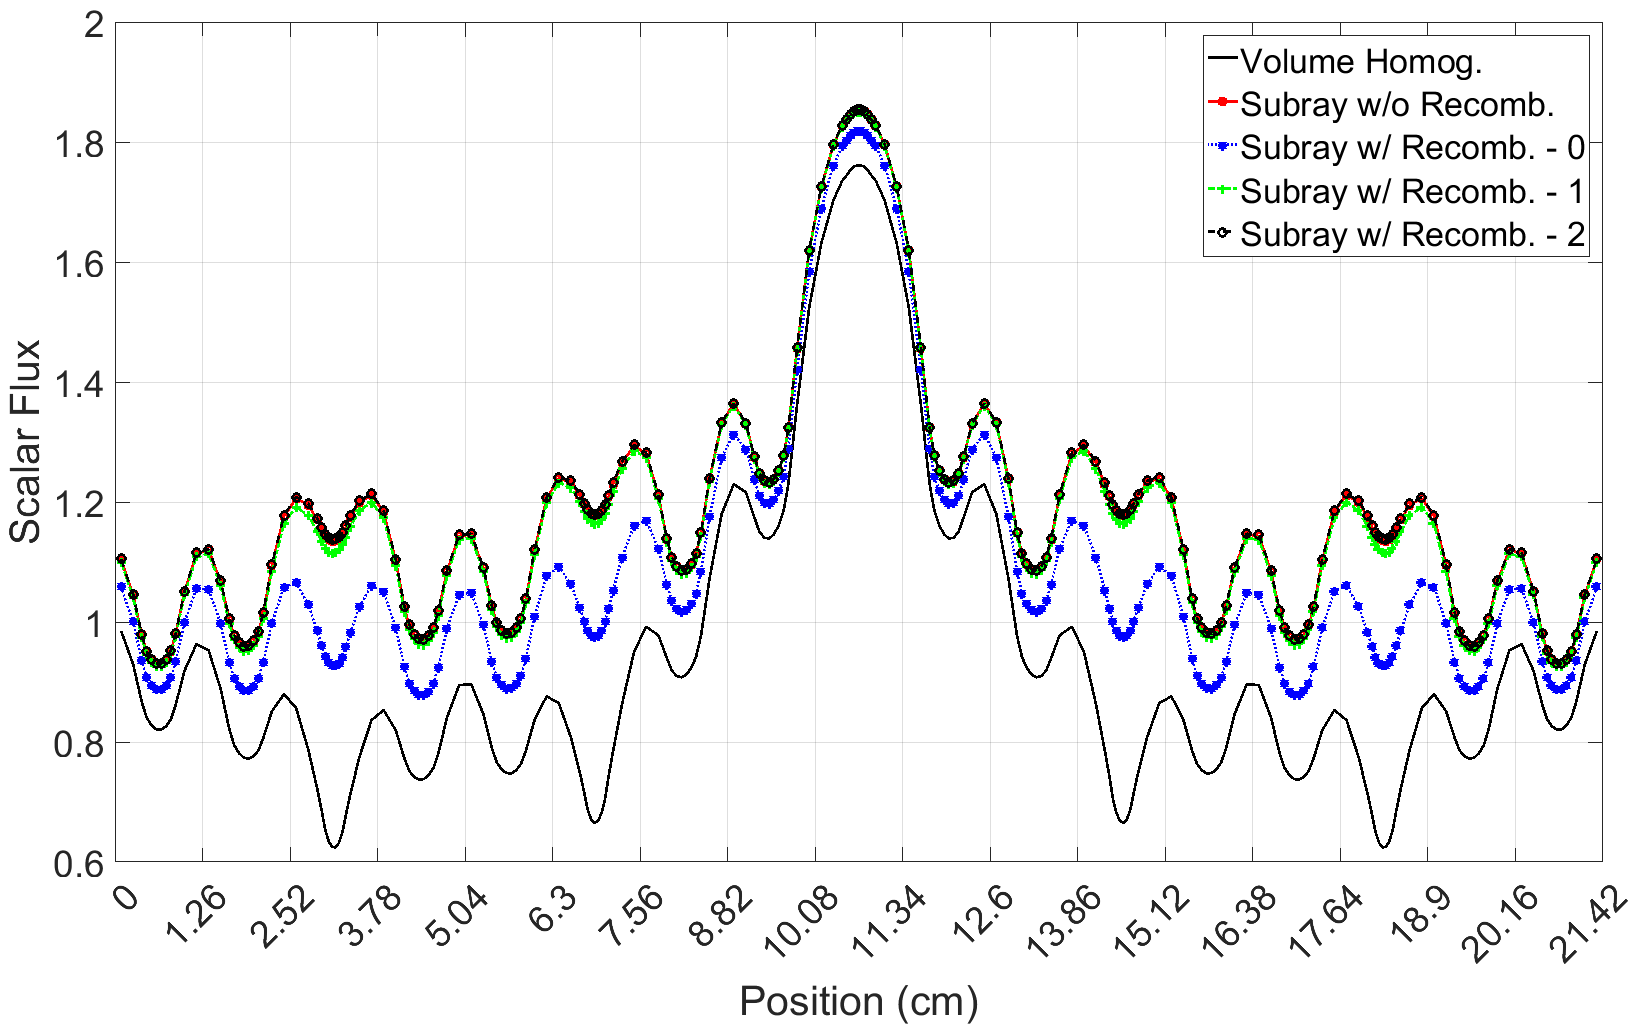
\includegraphics[width=\textwidth]{scalflux7.png}
    }
    \caption{Scalar flux distributions for 1D subray MOC calculations}\label{f:1d-subray-scalflux}
\end{figure}

In Figure \ref{f:1d-subray-keff}, the red line is subray without recombination, meaning that two completely separate solves were done each iteration and the resulting scalar fluxes were mixed using volume fractions.  The rodded and unrodded solves have separate angular flux boundary conditions which are saved for each subsequent iteration.  This provides the reference solution.  The volume homogenization solution is a traditional MOC calculation without treating the partially inserted rod.  As is evident, the errors from this method are large, nearing 15\% around 50-60\% withdrawal.  Using subray MOC in only the partially rodded pin cells, indicated in the figure by ``Subray w/ Recomb. - 0'', corrects a significant amount of the error and brings the maximum difference closer to 5\%.  Using a recombination factor of 1 means that subray is now used in all the pin cells between the control rods, correctly resolving the interference effects of the rods and eliminating almost all of the remaining error.  Finally, a recombination factor of 2 extends the subrays all the way to the problem boundary, effectively performing the same calculation as the reference solution.

In addition to the eigenvalue calculations, the scalar flux differences are shown for groups 1 and 7 at 50\% rod withdrawal in Figure \ref{f:1d-subray-scalflux}.  For both groups, it is evident that subray MOC effectively reduces the error caused by the partially inserted rod.  Only performing subray MOC in the rodded pin cells eliminates the majority of the error, but for both the eigenvalue and scalar flux distributions, it is necessary to delay recombination of the angular fluxes for at least one neighboring pin cell to capture the effects of the rod on the source in neighboring pin cells.  This effect is exaggerated by the 1D geometry since the solve is being performed exlusively in the direction that minimizes the distance between pins.  Furthermore, most PWR geometries have at least 2 pins between control rodlets, which further diminishes the effects of rod interference.  While these 1D results do not definitively indicate that recombination should be extended beyond the edge of the partially rodded pin cell, it is important to keep this in mind in the 2D and 3D calculations.

\subsection{2D C5G7}

\begin{figure}[h]
    \centering
    \subfigure{
        \centering
        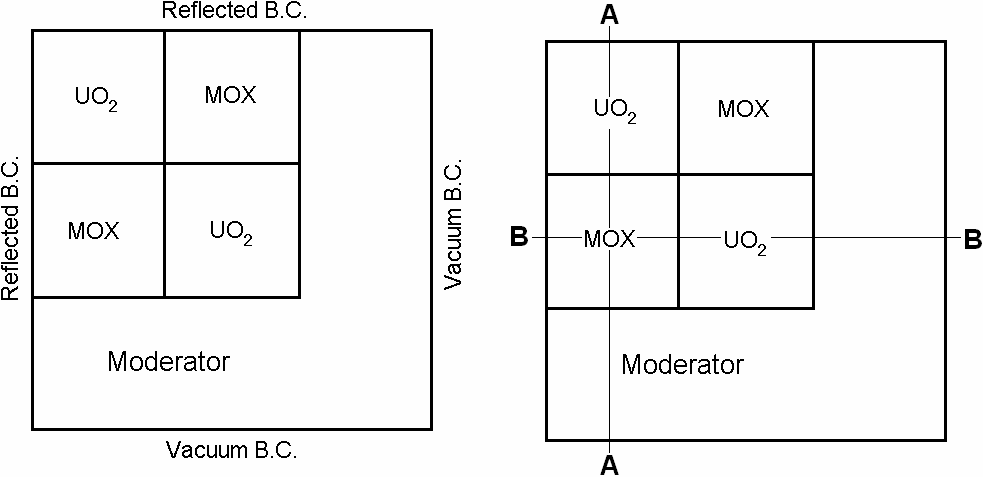
\includegraphics[width=0.8\textwidth]{c5g7-core-radial.png}
    }
    ~
    \subfigure{
        \centering
        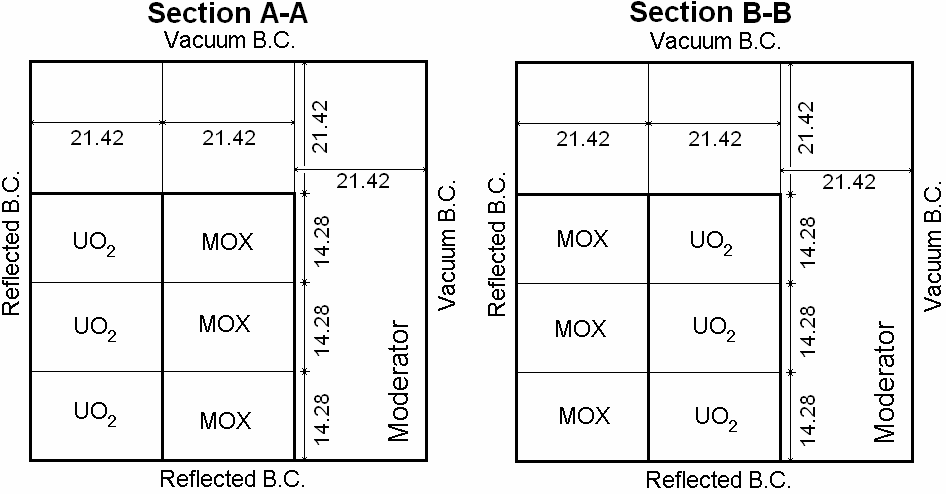
\includegraphics[width=0.8\textwidth]{c5g7-core-axial.png}
    }
    \caption[Descriptiong of C5G7 Core]{Description of C5G7 Core\cite{EELewisC5G7extended2005}}\label{f:c5g7-core}
\end{figure}

\begin{figure}[h]
    \centering
    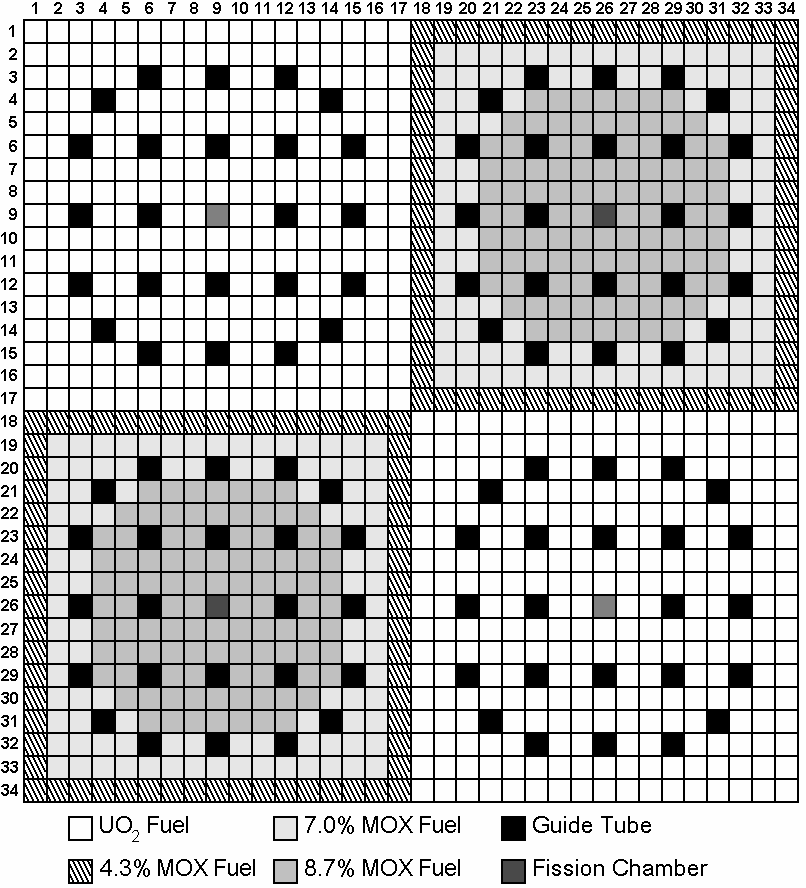
\includegraphics[width=0.8\textwidth]{c5g7-assemblies-radial.png}
    \caption[Description of C5G7 Assembly]{Description of C5G7 Assembly\cite{EELewisC5G7extended2005}}\label{f:c5g7-assemblies}
\end{figure}

To test the mechanics of subray MOC in MPACT, 2D variations of the C5G7 benchmark problems were used.  These problems consist of 17$\times$17 UO$_2$ and MOX assemblies with control rods and a radial reflector region.  Figure \ref{f:c5g7-core} shows an illustration of the core layout, and Figure \ref{f:c5g7-assemblies} shows the assembly layout.  This section will present results for subray MOC using 3 different 2D problems derived from these descriptions.

All calculations in this section used 0.03 cm ray spacing with 16 azmiuthal angles and 3 polar angles per octant.  A 1D P$_3$ solver was used for the subplane axial calculations unless otherwise noted.  The calculations were converged until the change in both the eigenvalue and fission source were less than $10^{-6}$.  All pin meshes in the fuel assemblies used 5 radial rings in the fuel, 2 rings in the moderator, and 8 azimuthal divisions in every radial region for a total of 64 flat source regions in each pin cell.  This mesh was also used for the rodded pin cells in the axial reflector region.  The remaining axial reflector pin cells and all radial reflector pin cells used a Cartesian grid with 5 x- and y- divisions, for a total of 25 equal-volume flat source regions.

\subsubsection{UO\texorpdfstring{$_2$}{2} Assembly}\label{sss:results-2d-assem}

\begin{table}[h]
    \centering
    \caption[2D C5G7 UO$_2$ Assembly Recombination Sensitivity]{2D C5G7 UO$_2$ assembly eigenvalue and power distribution differences for subray recombination parameter sensitivity.  A * indicates that finite difference was used axially instead of P$_3$}\label{t:c5g7-2d-asy-recomb}
    \resizebox{\textwidth}{!}{
        \begin{tabular}{l l l l l l l l l l l l l l}
        \toprule
        Rod & Reference & \multicolumn{3}{c}{Subray-0} & \multicolumn{3}{c}{Subray-1} & \multicolumn{3}{c}{Subray-2} & \multicolumn{3}{c}{Subray-3} \\
        Position & \keff{} & \keff{} & \multicolumn{2}{l}{Pin Powers} & \keff{} & \multicolumn{2}{l}{Pin Powers} & \keff{} & \multicolumn{2}{l}{Pin Powers} & \keff{} & \multicolumn{2}{l}{Pin Powers} \\
        &  &  & RMS & Max &  & RMS & Max &  & RMS & Max &  & RMS & Max \\
        \midrule
1* & 1.02535 & -23  & 0.05\% & 0.09\% & -59  & 0.06\% & 0.11\% & -58  & 0.06\% & 0.11\% & -58  & 0.06\% & 0.11\% \\
2 & 1.06065 & -117 & 0.11\% & 0.21\% & -121 & 0.11\% & 0.22\% & -120 & 0.11\% & 0.22\% & -120 & 0.11\% & 0.22\% \\
3 & 1.09578 & -165 & 0.14\% & 0.27\% & -175 & 0.15\% & 0.28\% & -175 & 0.15\% & 0.28\% & -174 & 0.15\% & 0.28\% \\
4 & 1.13011 & -200 & 0.15\% & 0.29\% & -219 & 0.16\% & 0.30\% & -218 & 0.16\% & 0.30\% & -217 & 0.16\% & 0.30\% \\
5 & 1.16334 & -223 & 0.15\% & 0.29\% & -249 & 0.17\% & 0.31\% & -248 & 0.17\% & 0.30\% & -247 & 0.17\% & 0.30\% \\
6 & 1.19557 & -235 & 0.14\% & 0.27\% & -265 & 0.16\% & 0.29\% & -264 & 0.16\% & 0.29\% & -264 & 0.16\% & 0.29\% \\
7 & 1.22711 & -237 & 0.13\% & 0.24\% & -269 & 0.15\% & 0.26\% & -269 & 0.14\% & 0.26\% & -269 & 0.14\% & 0.26\% \\
8 & 1.25858 & -231 & 0.11\% & 0.20\% & -263 & 0.13\% & 0.22\% & -262 & 0.12\% & 0.22\% & -262 & 0.12\% & 0.22\% \\
9* & 1.29131 & -216 & 0.09\% & 0.16\% & -236 & 0.10\% & 0.18\% & -235 & 0.10\% & 0.18\% & -235 & 0.10\% & 0.18\% \\
        \midrule
        Average &  -- & 183 & 0.12\% & 0.22\% & 206 & 0.13\% & 0.24\% & 205 & 0.13\% & 0.23\% & 205 & 0.13\% & 0.23\% \\
        \bottomrule
    \end{tabular}
    }
\end{table}


\begin{table}[h]
\centering
\caption[2D C5G7 UO$_2$ Assembly Results]{2D C5G7 UO$_2$ eigenvalue and power distribution differences for each decusping method.  A * indicates that finite difference was used axially instead of P$_3$}\label{t:c5g7-2d-asy-methods}
\resizebox{\textwidth}{!}{
    \begin{tabular}{l l l l l l l l l l l l l l}
    \toprule
    Rod & Reference & \multicolumn{3}{c}{Subray-0} & \multicolumn{3}{c}{None} & \multicolumn{3}{c}{Subplane} & \multicolumn{3}{c}{Subplane + CP} \\
    Position & \keff{} & \keff{} & \multicolumn{2}{l}{Pin Powers} & \keff{} & \multicolumn{2}{l}{Pin Powers} & \keff{} & \multicolumn{2}{l}{Pin Powers} & \keff{} & \multicolumn{2}{l}{Pin Powers} \\
    &  &  & RMS & Max &  & RMS & Max &  & RMS & Max &  & RMS & Max \\
    \midrule
1* & 1.02535 & -23  & 0.05\% & 0.09\% & -1210 & 0.70\% & 1.46\% & -361  & 0.20\% & 0.42\% & -696 & 0.34\% & 0.78\% \\
2 & 1.06065 & -117 & 0.11\% & 0.21\% & -3123 & 1.71\% & 3.55\% & -724  & 0.38\% & 0.78\% & -626 & 0.30\% & 0.65\% \\
3 & 1.09578 & -165 & 0.14\% & 0.27\% & -4777 & 2.49\% & 5.11\% & -937  & 0.46\% & 0.94\% & -574 & 0.26\% & 0.56\% \\
4 & 1.13011 & -200 & 0.15\% & 0.29\% & -6053 & 2.98\% & 6.09\% & -1033 & 0.47\% & 0.96\% & -522 & 0.23\% & 0.48\% \\
5 & 1.16334 & -223 & 0.15\% & 0.29\% & -6848 & 3.19\% & 6.47\% & -1046 & 0.44\% & 0.90\% & -465 & 0.20\% & 0.40\% \\
6 & 1.19557 & -235 & 0.14\% & 0.27\% & -7067 & 3.11\% & 6.26\% & -996  & 0.40\% & 0.81\% & -400 & 0.16\% & 0.33\% \\
7 & 1.22711 & -237 & 0.13\% & 0.24\% & -6588 & 2.73\% & 5.45\% & -897  & 0.34\% & 0.68\% & -327 & 0.13\% & 0.25\% \\
8 & 1.25858 & -231 & 0.11\% & 0.20\% & -5245 & 2.04\% & 4.03\% & -754  & 0.27\% & 0.54\% & -242 & 0.09\% & 0.18\% \\
9* & 1.29131 & -216 & 0.09\% & 0.16\% & -2803 & 1.01\% & 1.98\% & -561  & 0.19\% & 0.38\% & -146 & 0.05\% & 0.10\% \\
    \midrule
    Average & -- & 183 & 0.12\% & 0.22\% & 4857 & 2.22\% & 4.49\% & 812 & 0.35\% & 0.71\% & 444 & 0.20\% & 0.41\% \\
    \bottomrule
    \end{tabular}
}
\end{table}

The first 2D problem is a single UO$_2$ assembly with control rods added to it.  A similar procedure was followed as with the 1D calculations with the problem being simulated at 10\% increments during the rod withdrawal.  The reference for these calculations was generated by dividing the MOC plane into two separate planes with their boundary aligned with the control rod.  Comparisons could then be made between the decusping methods and the reference solution for \keff{} and the radial power distribution.

Table \ref{t:c5g7-2d-asy-recomb} shows the results for the 2D assembly case for recombination factor values of 0, 1, 2, and 3.  The results for both \keff{} and power distribution are best for the Subray-0 option, with average \keff{} differences less than 200 pcm and maximum power differences averaging 0.22\%.  This Subray-0 option actually performs better than the others likely due to the approximation of a constant radial shape for each subregion during the source calculations prior to the subray MOC calculation.  \hl{Discussion}.

Table \ref{t:c5g7-2d-asy-methods} compares the results of subray MOC with the sublpane-based decusping methods described earlier.  The polynomial method is not compared because the data required to use them fo C5G7 has not been generated.  The subplane decusping method performs better with CP than without, as expected.  Overall, its performance is good, reducing the maximum power error to around 0.5\% on average and reducing the \keff{} error from an average of almost 5\% to under 500 pcm.  However, the Subray-0 treatment performs better than the Subplane + CP method, \hl{Discussion}

This relationship between Subplane + CP and Subray-0 is expected.  Both of them are improving the solution in a single pin cell by solving the rodded and unrodded levels separately.  However, Subplane + CP does this after the MOC calculation, only improving the CMFD and 1D P$_3$ cross sections.  The Subray-0 calculation uses 2D MOC, which should provide a solution superior to 1D CP.  It also calculates improved radial currents, and improves the solution in pins neighboring the control rodlets by improving the angular flux exiting the rodded pin cells.  Thus, it is expected that Subray-0 would consistently provide a better solution than the Subplane + CP decusing method.

It should be noted at this point that certain calculations whose results are shown in these and following tables failed to converge using the axial P$_3$ solver.  This occurred for all calculations that had multiple planes or used the subplane scheme.  This is a known issue with the axial solvers caused by the interpolation of the radial TL source.  Whenever a thin plane is next to a thick plane and a very large change in the radial TL occurs from the thin plane to the thick plane, the quadratic interpolation of the radial TL can cause shapes that make the P$_3$ solver unstable.  This can be shown to be the source of the instability by limiting the magnitude of the linear and quadratic components of the shape.

One of the other MPACT developers is currently implementing a new solver that employs a different technique to solve the P$_3$ equations, and is expected to resolve this instability.  Since that solver is not yet ready for use and limiting the linear and/or quadratic moments of the radial TL interpolation can have significant effects on accuracy, the cases which did not converge for either the reference or decusping method calculations simply used diffusion-based NEM solver instead of the P$_3$ solver.  This provides a less accurate solution, but using it in cases with and without cusping allows for a fair assessment of methods being tested here without abandoning the axial solve altogether.  The results that used diffusion instead of P$_3$ will be denoted with an asterisk (*) in all tables in this section.

\begin{table}[h]
    \centering
    \caption{Long Ray Data for 2D C5G7 UO\texorpdfstring{$_2$}{2} Rodded Assembly}\label{t:subray-data-2dassembly}
    \begin{tabular}{l l l}\toprule
        Method & Long Rays per Plane & Increase \\\midrule
        Reference & 29480 & -- \\
        Subray-0 & 48440 & 64\% \\
        Subray-1 & 52832 & 79\% \\
        Subray-2 & 56304 & 91\% \\
        Subray-3 & 58960 & 100\% \\
        \bottomrule
    \end{tabular}
\end{table}

\begin{table}[h]
    \centering
    \caption{Average Performance and Convergence Data for C5G7 Rodded UO\texorpdfstring{$_2$}{2} Assembly}\label{t:subray-performance-2dassembly}
    \begin{tabular}{l l l l}\toprule
        Method & Iterations & Runtime (s) & Speedup \\\midrule
Reference     & 16.4 & 119 & --   \\
None          & 14.6 & 56 & 2.14 \\
Subplane      & 14.9 & 57 & 2.10 \\
Subplane + CP & 15.2 & 63 & 1.91 \\
Subray-0      & 14.9 & 94 & 1.27  \\
Subray-1      & 15.3 & 104 & 1.15 \\ 
Subray-2      & 15.4 & 109 & 1.09 \\ 
Subray-3      & 15.3 & 107 & 1.11 \\ 
        \bottomrule
    \end{tabular}
\end{table}

While the subray MOC method is more accurate than the previous decusping methods, it is also more expensive.  Table \ref{t:subray-data-2dassembly} shows the long ray data for the reference case and each variation of the subray MOC calculations.  The first column is the total number of long rays including those duplicated for subray MOC.  The second column shows the percent increase in the number of long rays.  This value can be used to approximate the savings obtained by using subray MOC to resolve partially inserted rods instead of 2 separate MOC planes.  For the single assembly case, it is expected that Subray-3 and the reference case would take about the same amount of time for each MOC sweep since every long ray was duplicated for Subray-3.

Table \ref{t:subray-performance-2dassembly} shows the convergence and runtime data for each decusping method averaged over all 9 rod positions. The speedup of each case is defined as the reference runtime divided by the comparison runtime.  Using Table \ref{t:subray-data-2dassembly}, we can approximate an expected speedup for each case by taking the number of long rays in the reference (2 MOC planes) and dividing by the number in the comparison case (1 MOC plane).  Doing this, we get expected speedups of 1.22, 1.12, 1.05, and 1.0 for Subray-0, Subray-1, Subray-2, and Subray-3, respectively.  The observed speedups are similar to, but consistently a little better than predicted.  Subray MOC takes between 1 and 1.5 iterations fewer, on average, than the reference case.  Furthermore, there is some small gain in efficiency from having all the long rays in a single sweep instead of two separate sweeps, though this is a smaller effect.  Thus, subray MOC performs about as well as expected for this implementation.  The other methods all see a speedup around 2.0, which is expected since the amount of time spent in MOC is exactly half that of the reference.  The differences in the CMFD solve and number of iterations introduce some variation in the speedup, which is to be expected.

\subsubsection{2D Core -- Rodded Center Assembly}

\begin{table}[h]
    \centering
    \caption[2D C5G7 Core Recombination Sensitivity, Center Assembly]{2D C5G7 center assembly rod withdrawal eigenvalue and pin power differences for subray recombination parameter sensitivity.  A * indicates that finite difference was used axially instead of P$_3$}\label{t:c5g7-2d-center-recomb}
    \resizebox{\textwidth}{!}{
        \begin{tabular}{l l l l l l l l l l l l l l}
            \toprule
            Rod & Reference & \multicolumn{3}{c}{Subray-0} & \multicolumn{3}{c}{Subray-1} & \multicolumn{3}{c}{Subray-2} & \multicolumn{3}{c}{Subray-3} \\
            Position & \keff{} & \keff{} & \multicolumn{2}{l}{Pin Powers} & \keff{} & \multicolumn{2}{l}{Pin Powers} & \keff{} & \multicolumn{2}{l}{Pin Powers} & \keff{} & \multicolumn{2}{l}{Pin Powers} \\
            &  &  & RMS & Max &  & RMS & Max &  & RMS & Max &  & RMS & Max \\
            \midrule
1* & 1.06839 & -15  & 0.10\% & 0.29\% & -15  & 0.10\% & 0.29\% & -15  & 0.10\% & 0.29\% & -15  & 0.10\% & 0.29\% \\
2 & 1.07746 & -33  & 0.22\% & 0.67\% & -34  & 0.22\% & 0.68\% & -34  & 0.22\% & 0.67\% & -34  & 0.22\% & 0.67\% \\
3 & 1.08777 & -53  & 0.32\% & 1.03\% & -56  & 0.34\% & 1.07\% & -55  & 0.34\% & 1.06\% & -55  & 0.34\% & 1.06\% \\
4 & 1.09919 & -72  & 0.41\% & 1.34\% & -78  & 0.45\% & 1.45\% & -78  & 0.45\% & 1.44\% & -78  & 0.45\% & 1.44\% \\
5 & 1.11160 & -89  & 0.46\% & 1.53\% & -99  & 0.51\% & 1.69\% & -98  & 0.50\% & 1.66\% & -98  & 0.50\% & 1.66\% \\
6 & 1.12495 & -102 & 0.49\% & 1.66\% & -115 & 0.55\% & 1.83\% & -115 & 0.54\% & 1.82\% & -115 & 0.54\% & 1.81\% \\
7 & 1.13925 & -112 & 0.49\% & 1.70\% & -127 & 0.55\% & 1.88\% & -126 & 0.55\% & 1.87\% & -126 & 0.55\% & 1.86\% \\
8 & 1.15469 & -117 & 0.47\% & 1.65\% & -133 & 0.53\% & 1.83\% & -132 & 0.53\% & 1.81\% & -132 & 0.52\% & 1.81\% \\
9* & 1.17190 & -117 & 0.43\% & 1.50\% & -127 & 0.46\% & 1.61\% & -126 & 0.46\% & 1.60\% & -126 & 0.46\% & 1.60\% \\
            \midrule
            Average & -- & 79 & 0.38\% & 1.26\% & 87 & 0.41\% & 1.37\% & 87 & 0.41\% & 1.36\% & 87 & 0.41\% & 1.36\% \\
            \bottomrule
        \end{tabular}
    }
\end{table}

\begin{table}[h]
    \centering
    \caption[2D C5G7 Core Results, Center Assembly]{2D C5G7 center assembly rod withdrawal eigenvalue and pin power differences for each decusping method.  A * indicates that finite difference was used axially instead of P$_3$}\label{t:c5g7-2d-center-methods}
    \resizebox{\textwidth}{!}{
        \begin{tabular}{l l l l l l l l l l l l l l}
            \toprule
            Rod & Reference & \multicolumn{3}{c}{Subray-0} & \multicolumn{3}{c}{None} & \multicolumn{3}{c}{Subplane} & \multicolumn{3}{c}{Subplane + CP} \\
            Position & \keff{} & \keff{} & \multicolumn{2}{l}{Pin Powers} & \keff{} & \multicolumn{2}{l}{Pin Powers} & \keff{} & \multicolumn{2}{l}{Pin Powers} & \keff{} & \multicolumn{2}{l}{Pin Powers} \\
            &  &  & RMS & Max &  & RMS & Max &  & RMS & Max &  & RMS & Max \\
            \midrule
1* & 1.06839 & -15  & 0.10\% & 0.29\% & -286  & 1.73 \% & 12.70\% & -87  & 0.52\% & 1.35\% & -169 & 0.99\% & 2.46\% \\
2 & 1.07746 & -33  & 0.22\% & 0.67\% & -811  & 4.75 \% & 21.30\% & -198 & 1.13\% & 3.06\% & -174 & 0.97\% & 2.57\% \\
3 & 1.08777 & -53  & 0.32\% & 1.03\% & -1369 & 7.71 \% & 29.42\% & -290 & 1.56\% & 4.42\% & -181 & 0.97\% & 2.70\% \\
4 & 1.09919 & -72  & 0.41\% & 1.34\% & -1918 & 10.33\% & 36.00\% & -360 & 1.83\% & 5.35\% & -185 & 0.94\% & 2.75\% \\
5 & 1.11160 & -89  & 0.46\% & 1.53\% & -2400 & 12.25\% & 39.83\% & -405 & 1.93\% & 5.84\% & -184 & 0.88\% & 2.68\% \\
6 & 1.12495 & -102 & 0.49\% & 1.66\% & -2738 & 13.12\% & 39.38\% & -424 & 1.89\% & 5.89\% & -174 & 0.78\% & 2.47\% \\
7 & 1.13925 & -112 & 0.49\% & 1.70\% & -2820 & 12.55\% & 32.80\% & -416 & 1.72\% & 5.52\% & -155 & 0.65\% & 2.11\% \\
8 & 1.15469 & -117 & 0.47\% & 1.65\% & -2478 & 10.08\% & 18.00\% & -377 & 1.44\% & 4.76\% & -124 & 0.48\% & 1.62\% \\
9* & 1.17190 & -117 & 0.43\% & 1.50\% & -1461 & 5.31 \% & 0.00 \% & -300 & 1.06\% & 3.60\% & -80  & 0.29\% & 1.00\% \\
            \midrule
            Average & -- & 79 & 0.38\% & 1.26\% & 1809 & 8.65\% & 25.49\% & 317 & 1.45\% & 4.42\% & 158 & 0.77\% & 2.26\% \\
            \bottomrule
        \end{tabular}
    }
\end{table}

The second problem uses the full radial core layout from Figures \ref{f:c5g7-core} and \ref{f:c5g7-assemblies}.  A control rod was added to the northwest UO$_2$ assembly, and the same procedure was followed as for the 2D assembly.  Table \ref{t:c5g7-2d-center-recomb} shows the results for subray MOC as a function of recombination value.  The trends observed in these results match more closely with expectations.  As the recombination factor is increased from 0 to 3, the errors monotically decrease.  The largest jump occurs from Subray-0 to Subray-1, and the smallest from Subray-2 to Subray-3.  This matches both physical intuition about the local effects of each control rodlet as well as the results of the 1D prototype subray MOC calculations.  The decrease in error from Subray-2 to Subray-3 might be slightly larger if the recombination were not restricted to the rodded assembly, as described by Figure \ref{f:recombination}.  However, the additional benefits from Subray-3 are likely insignificant when compared with the time to implement that logic and increased runtime of subray MOC.

Table \ref{t:c5g7-2d-center-methods} compares subray MOC to the other methods. The same observations can be made for these calculations as for the 2D assembly calculations.  The subplaned decusping is much better with CP than without, and subray MOC is better still, reducing the maximum power differences from around 25\% to less than 2\% for every rod position.  Furthermore, the \keff{} differences are reduced from almost around 2\% with no treatment and around 150 pcm with Subplane + CP to less than 100 pcm on average with Subray-0.

\begin{table}[h]
    \centering
    \caption{Long Ray Data for C5G7 Core}\label{t:subray-data-2dcore}
    \begin{tabular}{l l l }\toprule
        Method & Long Rays per Plane & Increase \\\midrule
        Reference & 88440 & -- \\
        Subray-0 & 107400 & 21\% \\
        Subray-1 & 111792 & 26\% \\
        Subray-2 & 115264 & 30\% \\
        Subray-3 & 117920 & 33\% \\
        \bottomrule
    \end{tabular}
\end{table}

\begin{table}[h]
    \centering
    \caption[2D C5G7 Core Performance Data, Center Assembly]{Average Performance and Convergence Data for 2D C5G7 Core with Rodded NW Assembly}\label{t:subray-performance-2dcoreNW}
    \begin{tabular}{l l l l}\toprule
        Method & Iterations & Runtime (s) & Speedup \\\midrule
Reference     & 25.7 & 1107 & --  \\
None          & 25.8 & 739 & 1.50 \\ 
Subplane      & 26.7 & 725 & 1.53 \\ 
Subplane + CP & 26.9 & 695 & 1.61 \\
Subray-0      & 26.4 & 861 & 1.29 \\ 
Subray-1      & 25.9 & 881 & 1.26 \\ 
Subray-2      & 26.1 & 920 & 1.21 \\ 
Subray-3      & 26.1 & 938 & 1.18 \\ 
        \bottomrule
    \end{tabular}
\end{table}

As with the single assembly, the long ray data can again be used to make some predictions about performance.  Because this problem has multiple assemblies and only one is partially rodded, the speedup observed for subray MOC is expected to be larger than that of the single assembly case.  Using the same procedure as for the assembly, we can predict approximate speedups of 1.65, 1.59, 1.54, and 1.50 for Subray-0, Subray-1, Subray-2, and Subray-3, respectively.  In this case the observed speedups are significantly worse than predicted, for several reasons.  First, subray MOC takes more iterations on average than the reference.  Second, the subplane CMFD and P$_3$ systems are the same size for all decusping methods as for the reference.  This was not important for the single assembly, but the 2D core is large enough that these other parts of the 2D/1D iteration can no longer be ignored in predicting the runtime.  However, in spite of these issues, a speedup of 20-30\% is still achieved with each of the subray MOC methods.

\subsubsection{2D Core -- Rodded Corner Assembly}

\begin{table}[h]
    \centering
    \caption[2D C5G7 Core Recombination Sensitivity, Corner Assembly]{2D C5G7 corner assembly rod withdrawal eigenvalue and pin power differences for subray recombination parameter sensitivity.  A * indicates that finite difference was used axially instead of P$_3$}\label{t:c5g7-2d-corner-recomb}
    \resizebox{\textwidth}{!}{
        \begin{tabular}{l l l l l l l l l l l l l l}
            \toprule
            Rod & Reference & \multicolumn{3}{c}{Subray-0} & \multicolumn{3}{c}{Subray-1} & \multicolumn{3}{c}{Subray-2} & \multicolumn{3}{c}{Subray-3} \\
            Position & \keff{} & \keff{} & \multicolumn{2}{l}{Pin Powers} & \keff{} & \multicolumn{2}{l}{Pin Powers} & \keff{} & \multicolumn{2}{l}{Pin Powers} & \keff{} & \multicolumn{2}{l}{Pin Powers} \\
            &  &  & RMS & Max &  & RMS & Max &  & RMS & Max &  & RMS & Max \\
            \midrule
1* & 1.18889 & -2  & 0.03\% & 0.11\% & -2  & 0.03\% & 0.11\% & -1  & 0.03\% & 0.11\% & -1  & 0.03\% & 0.11\% \\
2 & 1.18966 & -4  & 0.06\% & 0.23\% & -4  & 0.06\% & 0.23\% & -3  & 0.06\% & 0.23\% & -3  & 0.06\% & 0.23\% \\
3 & 1.19048 & -6  & 0.09\% & 0.33\% & -5  & 0.09\% & 0.34\% & -5  & 0.09\% & 0.33\% & -5  & 0.09\% & 0.33\% \\
4 & 1.19135 & -8  & 0.11\% & 0.40\% & -7  & 0.12\% & 0.42\% & -7  & 0.12\% & 0.41\% & -7  & 0.12\% & 0.41\% \\
5 & 1.19227 & -9  & 0.13\% & 0.45\% & -9  & 0.14\% & 0.47\% & -8  & 0.14\% & 0.47\% & -8  & 0.14\% & 0.47\% \\
6 & 1.19324 & -10 & 0.14\% & 0.47\% & -10 & 0.16\% & 0.50\% & -9  & 0.15\% & 0.50\% & -9  & 0.15\% & 0.50\% \\
7 & 1.19427 & -10 & 0.15\% & 0.47\% & -11 & 0.17\% & 0.51\% & -10 & 0.16\% & 0.51\% & -10 & 0.16\% & 0.51\% \\
8 & 1.19538 & -10 & 0.15\% & 0.46\% & -11 & 0.17\% & 0.50\% & -11 & 0.17\% & 0.50\% & -11 & 0.17\% & 0.50\% \\
9* & 1.19666 & -10 & 0.15\% & 0.42\% & -10 & 0.16\% & 0.44\% & -10 & 0.16\% & 0.44\% & -10 & 0.16\% & 0.44\% \\
            \midrule
            Average & -- & 8 & 0.11\% & 0.37\% & 7 & 0.12\% & 0.39\% & 7 & 0.12\% & 0.39\% & 7 & 0.12\% & 0.39\% \\
            \bottomrule
        \end{tabular}
    }
\end{table}

\begin{table}[h]
    \centering
    \caption[2D C5G7 Core Results, Corner Assembly]{2D C5G7 corner assembly rod withdrawal eigenvalue and pin power differences for each decusping method.  A * indicates that finite difference was used axially instead of P$_3$}\label{t:c5g7-2d-corner-methods}
    \resizebox{\textwidth}{!}{
        \begin{tabular}{l l l l l l l l l l l l l l}
            \toprule
            Rod & Reference & \multicolumn{3}{c}{Subray-0} & \multicolumn{3}{c}{None} & \multicolumn{3}{c}{Subplane} & \multicolumn{3}{c}{Subplane + CP} \\
            Position & \keff{} & \keff{} & \multicolumn{2}{l}{Pin Powers} & \keff{} & \multicolumn{2}{l}{Pin Powers} & \keff{} & \multicolumn{2}{l}{Pin Powers} & \keff{} & \multicolumn{2}{l}{Pin Powers} \\
            &  &  & RMS & Max &  & RMS & Max &  & RMS & Max &  & RMS & Max \\
            \midrule
1* & 1.18889 & -2  & 0.03\% & 0.11\% & -26  & 0.43\% & 1.35\% & -9  & 0.13\% & 0.42\% & -16 & 0.24\% & 0.73\% \\
2 & 1.18966 & -4  & 0.06\% & 0.23\% & -71  & 1.16\% & 3.57\% & -18 & 0.28\% & 0.88\% & -16 & 0.24\% & 0.74\% \\
3 & 1.19048 & -6  & 0.09\% & 0.33\% & -114 & 1.86\% & 5.67\% & -25 & 0.39\% & 1.19\% & -16 & 0.24\% & 0.74\% \\
4 & 1.19135 & -8  & 0.11\% & 0.40\% & -153 & 2.50\% & 7.48\% & -30 & 0.46\% & 1.38\% & -17 & 0.24\% & 0.73\% \\
5 & 1.19227 & -9  & 0.13\% & 0.45\% & -185 & 3.01\% & 8.84\% & -33 & 0.50\% & 1.47\% & -16 & 0.23\% & 0.70\% \\
6 & 1.19324 & -10 & 0.14\% & 0.47\% & -205 & 3.32\% & 9.58\% & -34 & 0.51\% & 1.47\% & -15 & 0.22\% & 0.64\% \\
7 & 1.19427 & -10 & 0.15\% & 0.47\% & -207 & 3.33\% & 9.43\% & -33 & 0.49\% & 1.39\% & -13 & 0.19\% & 0.55\% \\
8 & 1.19538 & -10 & 0.15\% & 0.46\% & -182 & 2.89\% & 7.98\% & -30 & 0.45\% & 1.22\% & -11 & 0.15\% & 0.43\% \\
9* & 1.19666 & -10 & 0.15\% & 0.42\% & -110 & 1.71\% & 4.61\% & -24 & 0.36\% & 0.96\% & -7  & 0.10\% & 0.27\% \\
            \midrule
            Average & -- & 8 & 0.11\% & 0.37\% & 139 & 2.25\% & 6.50\% & 26 & 0.40\% & 1.15\% & 14 & 0.21\% & 0.61\% \\
            \bottomrule
        \end{tabular}
    }
\end{table}

The final 2D problem is the same as the previous one, except that the southeast corner UO$_2$ assembly is rodded instead of the northwest assembly.  Tables \ref{t:c5g7-2d-corner-recomb} and \ref{t:c5g7-2d-corner-methods} show similar results to the previous two problems.  For all methods, the errors are lower for this problem than for the first multi-assembly problem.  There are two reasons for this.  First, the control rods for this problem are in a lower power region than for the previous one, so the absolute differences in power are sure to be smaller for any decusping method.  Second, the rodded assembly is not next to reflecting boundary conditions.  In the previous problem, if the reflecting boundary conditions are accounted for, there are effectively 4 rodded assemblies in a cluster in the center of the core.  However, all subrays are forced to recombine at the problem boundary, a decision which is not necessary but was made for the sake of code simplicity and time.  This likely has at least some negative impact on the results of the previous problem.  The rodded assembly in this problem is surrounded by unrodded assemblies that do not require subray MOC, removing one approximation that was forced by the other problem.

\begin{table}[h]
    \centering
    \caption[2D C5G7 Core Performance Data, Corner Assembly]{Average Performance and Convergence Data for 2D C5G7 Core with Rodded SE Assembly}\label{t:subray-performance-2dcoreSE}
    \begin{tabular}{l l l l}\toprule
        Method & Iterations & Runtime (s) & Speedup \\\midrule
Reference     & 24.4 & 1006 & --  \\
None          & 24.0 & 657 & 1.54 \\
Subplane      & 25.3 & 636 & 1.59 \\
Subplane + CP & 25.3 & 629 & 1.60 \\
Subray-0      & 25.3 & 798 & 1.26 \\
Subray-1      & 25.0 & 833 & 1.21 \\
Subray-2      & 25.0 & 855 & 1.18 \\
Subray-3      & 25.0 & 878 & 1.15 \\
        \bottomrule
    \end{tabular}
\end{table}

The primary reason to show this problem is that because the rods are in the center of the model, the long rays duplicated for the subray MOC calculation are longer for some angles, especially those between the northeast and southwest corners of the model.  Thus, while the total number of rays duplicated is the same as for the previous problem (Table \ref{t:subray-data-2dcore}), the amount of work done for the duplicated rays is different.  This will show what, if any, impact the position of the control rods in the core could have on the efficiency of the subray MOC calculations.

Table \ref{t:subray-performance-2dcoreSE} shows the convergence and runtime data for this problem.  Compared with the previous 2D core problem, the speedups are similar, but lower by about 0.03 for each subray MOC calculation.  The convergence behavior of this problem is similar to the previous one, so this small decrease in speedup is likely due to duplicating longer core rays.  Overall, the impact of the control rod locations has a negligible impact on the speedups observed by using subray MOC or the other decusping methods.

\subsection{3D C5G7}

\subsubsection{3D C5G7 UO\texorpdfstring{$_2$}{2} Assembly}

One 3D problem was also used to test subray MOC.  This problem consists of the NW UO$_2$ assembly.  As shown in Figure \ref{f:c5g7-core}, this assembly has a 42.84 cm active fuel height with a 21.42 cm axial reflector on top.  The control rods at full insertion extend from the bottom of the active fuel all the way to the top of the reflector.  In MPACT, this was modeled using 4 MOC planes: 3 in the active fuel region and 1 for the axial refelctor.  The rod was withdrawn from the bottom of the fuel to the top in 30 steps of 1.428 cm.  At each position, a reference solution was generated using the same method as the 2D calculations by adding an extra MOC plane boundary that aligned with the rod position to eliminate all cusping effects.

\begin{table}
    \centering
    \caption[3D C5G7 UO$_2$ Assembly Recombination Sensitivity]{3D C5G7 UO$_2$ assembly rod withdrawal eigenvalue and pin power difference summary}\label{t:c5g7-3d-assembly}
    \begin{tabular}{l l l l}\toprule
        \multirow{2}{*}{Method} & \keff{} & \multicolumn{2}{l}{Pin Powers} \\
         & Diff. & RMS & Max \\\midrule
None        & 2193 & 6.05\% & 10.95\% \\
Subplane    & 222  & 0.88\% &  1.64\% \\
Subplane+CP & 114  & 0.45\% &  0.84\% \\
Subray-0    & 52   & 0.25\% &  0.54\% \\
Subray-1    & 56   & 0.25\% &  0.55\% \\
Subray-2    & 56   & 0.25\% &  0.54\% \\
Subray-3    & 56   & 0.25\% &  0.54\% \\
         \bottomrule
    \end{tabular}
\end{table}

Table \ref{t:c5g7-3d-assembly} shows the average errors for each method for the 3D assembly.  For this problem, the trends from the 2D calculations are not observed.  The subray MOC results are consistently better than the subplane method without CP.  However, with CP, the subplane method is signficantly better than subray MOC.  Furthermore, the \keff{} errors decrease with increasing recombination factor, but the power distribution errors increase.  While the results with subray MOC are still fairly good compared with no treatment, the Subplane + CP method is clearly the most effective for this problem.  It is expected that this error comes from interactions between subray MOC and the 1D P$_3$ solver that are not an issue in the 2D calculations, making it likely that some improvements could be made to this iteration scheme improve the subray MOC results.

\begin{table}[h]
    \centering
    \caption[3D C5G7 UO$_2$ Assembly Performance]{Average Performance and Convergence Data for 3D C5G7 Rodded UO$_2$ Assembly}\label{t:subray-performance-3Dassembly}
    \begin{tabular}{l l l l}\toprule
        Method & Iterations & Runtime (s) & Speedup \\\midrule
Reference     & 27.7 & 610 & --   \\
None          & 31.7 & 574 & 1.14 \\
Subplane      & 29.0 & 430 & 1.45 \\
Subplane + CP & 28.7 & 411 & 1.52 \\
Subray-0      & 28.1 & 526 & 1.19 \\
Subray-1      & 33.0 & 633 & 1.00 \\
Subray-2      & 30.4 & 599 & 1.04 \\
Subray-3      & 32.6 & 619 & 1.03 \\
        \bottomrule
    \end{tabular}
\end{table}

The 3D assembly has the same long ray parameters as those shown in Table \ref{t:subray-data-2dassembly} for the 2D assembly.  For the plane with the rod, the number of long rays matches with the subray entries of the table, while for the remaining planes the number of long rays matches the reference entry.  Because of this, the subray MOC calculation runtimes should be closer to the subplane calculation times than to the reference calculation, since 3 of the 4 planes are the same as the reference case.  Table \ref{t:subray-performance-3Dassembly} shows the convergence and runtime results for each of the methods.  The speedup for subray MOC is good compared to the reference for Subray-0.  Subray-3 shows virtually no speedup, which is expected since all long rays are duplicated in this problem.  However, Subray-1 and Subray-2 show little to no speedup.  This is due primarily to the increase in the number of iterations.  Many of the rod positions were difficult to converge, compared with the 2D calculations, reducing the speedup observed in this problem.

\subsubsection{3D Core -- Rodded Center Assembly}

\begin{table}
    \centering
    \caption[3D C5G7 Core with Rodded Center Assembly Results]{3D C5G7 core with rodded center assembly rod withdrawal eigenvalue and pin power difference summary}\label{t:c5g7-3d-core-center}
    \begin{tabular}{l l l l}\toprule
        \multirow{2}{*}{Method} & \keff{} & \multicolumn{2}{l}{Pin Powers} \\
        & Diff. & RMS & Max \\\midrule
None        & 21 & 6.62\% & 29.30\% \\
Subplane    & 21 & 0.69\% & 3.47 \% \\
Subplane+CP & 21 & 0.34\% & 1.69 \% \\
Subray-0    & 21 & 0.20\% & 1.06 \% \\
Subray-1    & 25 & 0.20\% & 1.14 \% \\
Subray-2    & 25 & 0.20\% & 1.11 \% \\
Subray-3    & 21 & 0.20\% & 1.11 \% \\
        \bottomrule
    \end{tabular}
\end{table}

\hl{discussion}

\begin{table}[h]
    \centering
    \caption[3D C5G7 Core with Rodded Center Assembly Performance]{Average Performance and Convergence Data for 3D C5G7 Core with Rodded Center  Assembly}\label{t:subray-performance-3Dcore-center}
    \begin{tabular}{l l l l}\toprule
        Method & Iterations & Runtime (s) & Speedup \\\midrule
        Reference     & 27.8 & 3156 & -- \\
        None          & 28.2 & 2936 & 1.34 \\
        Subplane      & 29.1 & 2363 & 1.34 \\
        Subplane + CP & 28.9 & 2814 & 1.13 \\
        Subray-0      & 28.8 & 3251 & 0.98 \\
        Subray-1      & 28.9 & 3204 & 0.99 \\
        Subray-2      & 29.1 & 3320 & 0.96 \\
        Subray-3      & 29.2 & 3352 & 0.94 \\
        \bottomrule
    \end{tabular}
\end{table}

\hl{discussion}

\subsubsection{3D Core -- Rodded Corner Assembly}

\begin{table}
\centering
\caption[3D C5G7 Core with Rodded Corner Assembly]{3D C5G7 core with rodded corner assembly rod withdrawal eigenvalue and pin power difference summary}\label{t:c5g7-3d-core-corner}
\begin{tabular}{l l l l}\toprule
    \multirow{2}{*}{Method} & \keff{} & \multicolumn{2}{l}{Pin Powers} \\
    & Diff. & RMS & Max \\\midrule
None        & 72 & 1.53\% & 7.01\% \\
Subplane    & 8  & 0.18\% & 1.08\% \\
Subplane+CP & 4  & 0.09\% & 0.56\% \\
Subray-0    & 2  & 0.05\% & 0.35\% \\
Subray-1    & 2  & 0.06\% & 0.37\% \\
Subray-2    & 2  & 0.06\% & 0.37\% \\
Subray-3    & 2  & 0.06\% & 0.37\% \\
    \bottomrule
\end{tabular}
\end{table}

\hl{discussion}

\begin{table}[h]
    \centering
    \caption[3D C5G7 Core with Rodded Corner Assembly Performance]{Average Performance and Convergence Data for 3D C5G7 Core with Rodded Corner  Assembly}\label{t:subray-performance-3Dcore-corner}
    \begin{tabular}{l l l l}\toprule
        Method & Iterations & Runtime (s) & Speedup \\\midrule
        Reference     & 27.2 & 3346 & --   \\
        None          & 27.0 & 2751 & 1.22 \\
        Subplane      & 28.2 & 2716 & 1.18 \\
        Subplane + CP & 28.2 & 2751 & 1.17 \\
        Subray-0      & 27.9 & 3115 & 1.08 \\
        Subray-1      & 28.1 & 3099 & 1.08 \\
        Subray-2      & 28.1 & 3132 & 1.07 \\
        Subray-3      & 28.2 & 3155 & 1.06 \\
        \bottomrule
    \end{tabular}
\end{table}

\hl{discussion}